\newcommand{\mainprogram}[0]{}
\documentclass[10pt]{article}

%packages +  bib
\usepackage[left=2.5cm,right=2.5cm,bottom=2cm,top=3.0cm]{geometry}
\usepackage{amsmath}      %std package for many operators
\usepackage{amssymb}      %symbolds i guess
\usepackage{bbold}	  %identity matrix
\usepackage{ dsfont }	  % i have no idea
\usepackage{color}              % for comments
\usepackage{xcolor}	   %for additional color, can be deleted in the end i think!!!s
\usepackage{physics}          % bra ket notation
\usepackage{slashed}          %for slash notation
\usepackage{fancyhdr}       %allows chance of layout
\usepackage[subfigure]{tocloft}    %TOC layout
\usepackage{indentfirst}      %for parindent after new section
\usepackage{graphicx,subfigure}	  %for uni logo
\usepackage{setspace}      %for spacing between the lines
\usepackage{simplewick}   %for wick contractions
\usepackage{tikz-feynman} %SM diagrams
\usepackage[title,titletoc]{appendix} %appendix written in table of contents
\usepackage[sorting=none]{biblatex}  %numbers of citation are how they appear in tex
\bibliography{literature.bib}

%Layout including how to enumberate equations
\setlength\parindent{0.8cm}
\setlength{\cftsecnumwidth}{35pt}
\setlength{\cftsubsecnumwidth}{35pt}
\pagestyle{fancy} %benutzerdef
\fancyhf{}
\fancyhead[R]{\thepage}
\renewcommand{\headrulewidth}{0pt}

\renewcommand{\thesection}{\Roman{section}} % i removed the ``.'' in the end ( in subsection it is still there) for references. It should work this way.
\renewcommand{\thesubsection}{\Alph{subsection}}
\renewcommand{\thesubsubsection}{\Alph{subsection}.\roman{subsubsection}}



\numberwithin{equation}{section}
\renewcommand{\theequation}{\arabic{section}.\arabic{equation}}

\renewcommand{\baselinestretch}{1.25}

%Additional Layout matters
\newcommand{\remark}[1]{\newline\newline \emph{#1} \newline\newline}

%dates


%Other / Names
\newcommand{\Mat}{\text{\emph{Mathematica}}}


%References
\newcommand{\howtowriteequation}{eq.$~$}
\newcommand{\cref}[1]{eq.$~$(#1)} % cite equation from other paper ref
\newcommand{\eref}[1]{\howtowriteequation (\ref{#1})}
\newcommand{\doubleref}[2]{\howtowriteequation (\ref{#1}, \ref{#2})}
\newcommand{\tripleref}[3]{\howtowriteequation (\ref{#1}, \ref{#2}, \ref{#3})}
\newcommand{\ereffromto}[2]{\howtowriteequation (\ref{#1})-(\ref{#2})}

\newcommand{\sref}[1]{section$~$\ref{#1}}
\newcommand{\Sref}[1]{Section$~$\ref{#1}}
\newcommand{\tref}[1]{table$~$\ref{#1}}
\newcommand{\fref}[1]{figure$~$\ref{#1}}
\newcommand{\aref}[1]{appendix$~$\ref{#1}}

\newcommand{\pref}[1]{page$~$\pageref{#1}}

\newcommand{\mc}[1]{\cite{#1}}

%Notes for correcting
\newcommand{\COM}[1]{\text{\textcolor{red}{#1}}}
\newcommand{\LBL}[0]{\COM{Hier}}
\newcommand{\spacee}{~~~~~~~}
%newline in formula with term exeeding length of a line
\newcommand{\nl}{\\&~~~}

%Functions and symbols
\newcommand{\gf}{G}
\newcommand{\hamiltonian}{H}
\newcommand{\flnso}{Op.}
\newcommand{\propagator}{\Delta}  % propagator symbol

%Fields (quark, gauge etc)
\newcommand{\Aqu}{B} %quantum gauge field
%operators
\newcommand{\operatorO}{O}
\newcommand{\twoq}[1]{\operatorO_q^{#1}}
\newcommand{\twoqbar}[1]{\overline \operatorO_{q}^{#1}}
\newcommand{\twog}[1]{\operatorO_{g}^{#1}}
\newcommand{\twogbar}[1]{\overline \operatorO_{g}^{#1}}

%Differential Operators
\newcommand{\dx}{\text{d}}
\newcommand{\abdif}[1]{\frac{\dx}{\dx #1  } }
\newcommand{\abdifof}[2]{\frac{\dx #1}{\dx #2  } }
\newcommand{\padif}[1]{\frac{\partial}{\partial #1  } }
\newcommand{\doublepadif}[2]{\frac{\partial^2}{\partial #1 \partial #2}}
\newcommand{\padifntimes}[2]{\frac{\partial^{#2}}{\partial #1^{#2}}}
\newcommand{\ft}{F}%field tensor
\newcommand{\cov} {D}
\newcommand{\covleft}{\overleftarrow{\cov}}
\newcommand{\covright}{\overrightarrow{\cov}}
\newcommand{\dxabc}{\left[\dx \alpha \dx \beta \dx \gamma\right]}
\newcommand{\dxabcprime}{\left[\dx \alpha' \dx \beta' \dx \gamma'\right]}
\newcommand{\dxfm}[2]{\frac{\dx^{#2}#1}{\left(2\pi\right)^{#2}}}
\newcommand{\dxfs}[2]{\dx^{#2}#1}
\newcommand{\ddx}{\dx ^d}


%Michelaneous including spinors
\newcommand{\metric}{\eta}
\newcommand{\idm}{{1}}
\newcommand{\abelian}[2]{\left[ #1, #2 \right]}
\newcommand{\expo}{e}
\newcommand{\skp}[2]{(#1|#2)}
\newcommand{\skpt}[2]{(#1\cdot#2)}
\newcommand{\spp}[1]{\langle #1 \rangle}
\newcommand{\aspp}[1]{\left[ #1 \right]}
\renewcommand{\trace}[0]{\text{Tr}}

%spinors
\newcommand{\psibar}{\overline\psi}
\newcommand{\psibarc}{\psibar_c}
\newcommand{\psibarq}{\psibar_q}
\newcommand{\psic}{\psi_c}
\newcommand{\psiq}{\psi_q}
\newcommand{\psip}{\psi_{+}}
\newcommand{\psim}{\psi_{-}}
\newcommand{\psit}{\overline\psi}
\newcommand{\chit}{\overline\chi}
\newcommand{\psipt}{\psit_{+}}
\newcommand{\psimt}{\psit_{-}}
\newcommand{\chip}{\chi_{+}}
\newcommand{\chim}{\chi_{-}}
\newcommand{\chipt}{\chit_{+}}
\newcommand{\chimt}{\chit_{-}}
\newcommand{\ispace}{~\hspace{-3pt}}
\newcommand{\ospex}{O}
\newcommand{\spideriv}[2]{\frac{#1\partial}{\partial #2}}
\newcommand{\spiderivb}[3]{\left(\spideriv{#1}{#2}\right)^{#3}}
\newcommand{\fbar}{\overline f}
\newcommand{\SX}{J}

%%Spinor Combinations
\newcommand{\lol}{\lambda\overline\lambda}
\newcommand{\mom}{\mu\overline\mu}
\newcommand{\lom}{\lambda\overline\mu}
\newcommand{\mol}{\mu\overline\lambda}
\newcommand{\olom}{\overline\lambda\overline\mu}
\newcommand{\omol}{\overline\mu\overline\lambda}
\newcommand{\om}{\overline\mu}
\newcommand{\ol}{\overline\lambda}
%skp that appear quite often such that the order is consistent
\newcommand{\skpyP}{\skp{y}{P}}
\newcommand{\skpPy}{\skpyP}

\newcommand{\skpyS}{\skp{y}{S}}
\newcommand{\skpSy}{\skpyS}
% q Bar, bold B , pplus, nbar
\newcommand{\qbar}{\overline q}
\newcommand{\bb}{\boldsymbol{b}}
\newcommand{\pp}{p_{+}}
\newcommand{\pphat}{\hat p_{+}}
\newcommand{\nbar}{\tilde n}
%Imaginary Unity, coupling: 
\newcommand{\imag}{\text{i}}
\newcommand{\as}{\alpha_s}
%Operators
%Wilson line, pretzelosity , Matrix element PS
\newcommand{\brez}{h_{1T}^{\bot}}
\newcommand{\wil}[2]{\left[#1,#2 \right]}
\newcommand{\myState}{P,S}
\newcommand{\fme}[1]{\bra{\myState}#1\ket{\myState}}
\newcommand{\twist}{T}
%O Gamma operators
\newcommand{\oga}{O ^{\Gamma  }}
\newcommand{\ogmu}{O^{\gamma^\mu}}
\newcommand{\ogmugfive}{O^{\gamma^\mu \gamma^5}}
\newcommand{\osigma}{O^{\imag \sigma ^{\mu \nu }\gamma_5}}
\newcommand{\ogplus}{O^{\gamma^{+}}}
\newcommand{\ogplusgfive}{O^{\gamma^{+} \gamma^5}}
\newcommand{\osigmaplus}{O^{\imag \sigma ^{\alpha + }\gamma_5}}
\newcommand{\osigmavarplus}[1]{O^{\imag \sigma ^{#1 + }\gamma_5}}
%3point operators
\newcommand{\ttp}{\mathcal{T}^\Gamma}
\newcommand{\ttpg}{\mathcal{T}^{\gamma_+}}
\newcommand{\ttpgg}{\mathcal{T}^{\gamma_+\gamma_5}}
\newcommand{\ttpsg}{\mathcal{T}^{\imag \sigma^{\alpha + }\gamma^5}}
\newcommand{\ttpsgadaptive}[3]{\mathcal{T}^{\imag \sigma^{#1 #2}\gamma^5}_{#3}}
%matrix elements of 3 point operators
\newcommand{\Dt}{\Delta T}
\newcommand{\Dtx}{\Dt (x_1,x_2,x_3)}
\newcommand{\Dtt}{\Delta \tilde T}
\newcommand{\dttg}{\delta \tilde T_g}
\newcommand{\dtte}{\delta \tilde T_\expsilon}
\newcommand{\dTe}{\delta T _\epsilon}
\newcommand{\dTex}{\delta T _\epsilon(x_1,x_2,x_3)}
\newcommand{\dTg}{\delta T _g}
\newcommand{\dTgx}{\delta T _g(x_1,x_2,x_3)}
\newcommand{\xonetwothree}{x_{1,2,3}}
%U gamma operators or full TMD s
\newcommand{\uga}{\mathcal{U}^{\Gamma}}
\newcommand{\udis}{\mathcal{U}_{DIS}^{\Gamma}}
\newcommand{\udy}{\mathcal{U}_{DY}^{\Gamma}}
\newcommand{\udygplus}{\mathcal{U}_{DY}^{\gamma^+}}
\newcommand{\udygplusgfive}{\mathcal{U}_{DY}^{\gamma^+\gamma_5}}
\newcommand{\udysg}{\mathcal{U}_{DY}^{\imag \sigma^{\alpha +}_{T} \gamma_5}}

\newcommand{\nameofO}{O}	
\newcommand{\ogt}{\nameofO_{TMD}^{\Gamma}}
\newcommand{\ogtfields}[2]{\nameofO_{#1}^{#2}}
\newcommand{\ogpt}{\nameofO_{TMD}^{\gamma_+}}

%phi distributions
\newcommand{\phiqh}{\Phi_{q\leftarrow h}}
\newcommand{\phiqhij}{\Phi_{q\leftarrow h,ij}}
\newcommand{\phiG}{\Phi_{q\leftarrow h}^{[\Gamma]}}
\newcommand{\phig}{\Phi_{q\leftarrow h}^{[\gamma^+]}}
\newcommand{\phigg}{\Phi_{q\leftarrow h}^{[\gamma^+ \gamma_5]}}
\newcommand{\phisg}[1]{\Phi_{q\leftarrow h}^{[\sigma^{#1 +}\gamma_5]}}

%Parametrization fucntions
\newcommand{\paraA}{A}
\newcommand{\paraB}{B}


%Graphics

\usepackage[]{hyperref}

\begin{document}


\ifdefined\mainprogram{}
\else
\documentclass[10pt]{article}

%packages +  bib
\usepackage[left=2.5cm,right=2.5cm,bottom=2cm,top=3.0cm]{geometry}
\usepackage{amsmath}      %std package for many operators
\usepackage{amssymb}      %symbolds i guess
\usepackage{bbold}	  %identity matrix
\usepackage{ dsfont }	  % i have no idea
\usepackage{color}              % for comments
\usepackage{xcolor}	   %for additional color, can be deleted in the end i think!!!s
\usepackage{physics}          % bra ket notation
\usepackage{slashed}          %for slash notation
\usepackage{fancyhdr}       %allows chance of layout
\usepackage[subfigure]{tocloft}    %TOC layout
\usepackage{indentfirst}      %for parindent after new section
\usepackage{graphicx,subfigure}	  %for uni logo
\usepackage{setspace}      %for spacing between the lines
\usepackage{simplewick}   %for wick contractions
\usepackage{tikz-feynman} %SM diagrams
\usepackage[title,titletoc]{appendix} %appendix written in table of contents
\usepackage[sorting=none]{biblatex}  %numbers of citation are how they appear in tex
\bibliography{literature.bib}

%Layout including how to enumberate equations
\setlength\parindent{0.8cm}
\setlength{\cftsecnumwidth}{35pt}
\setlength{\cftsubsecnumwidth}{35pt}
\pagestyle{fancy} %benutzerdef
\fancyhf{}
\fancyhead[R]{\thepage}
\renewcommand{\headrulewidth}{0pt}

\renewcommand{\thesection}{\Roman{section}} % i removed the ``.'' in the end ( in subsection it is still there) for references. It should work this way.
\renewcommand{\thesubsection}{\Alph{subsection}}
\renewcommand{\thesubsubsection}{\Alph{subsection}.\roman{subsubsection}}



\numberwithin{equation}{section}
\renewcommand{\theequation}{\arabic{section}.\arabic{equation}}

\renewcommand{\baselinestretch}{1.25}

%Additional Layout matters
\newcommand{\remark}[1]{\newline\newline \emph{#1} \newline\newline}

%dates


%Other / Names
\newcommand{\Mat}{\text{\emph{Mathematica}}}


%References
\newcommand{\howtowriteequation}{eq.$~$}
\newcommand{\cref}[1]{eq.$~$(#1)} % cite equation from other paper ref
\newcommand{\eref}[1]{\howtowriteequation (\ref{#1})}
\newcommand{\doubleref}[2]{\howtowriteequation (\ref{#1}, \ref{#2})}
\newcommand{\tripleref}[3]{\howtowriteequation (\ref{#1}, \ref{#2}, \ref{#3})}
\newcommand{\ereffromto}[2]{\howtowriteequation (\ref{#1})-(\ref{#2})}

\newcommand{\sref}[1]{section$~$\ref{#1}}
\newcommand{\Sref}[1]{Section$~$\ref{#1}}
\newcommand{\tref}[1]{table$~$\ref{#1}}
\newcommand{\fref}[1]{figure$~$\ref{#1}}
\newcommand{\aref}[1]{appendix$~$\ref{#1}}

\newcommand{\pref}[1]{page$~$\pageref{#1}}

\newcommand{\mc}[1]{\cite{#1}}

%Notes for correcting
\newcommand{\COM}[1]{\text{\textcolor{red}{#1}}}
\newcommand{\LBL}[0]{\COM{Hier}}
\newcommand{\spacee}{~~~~~~~}
%newline in formula with term exeeding length of a line
\newcommand{\nl}{\\&~~~}

%Functions and symbols
\newcommand{\gf}{G}
\newcommand{\hamiltonian}{H}
\newcommand{\flnso}{Op.}
\newcommand{\propagator}{\Delta}  % propagator symbol

%Fields (quark, gauge etc)
\newcommand{\Aqu}{B} %quantum gauge field
%operators
\newcommand{\operatorO}{O}
\newcommand{\twoq}[1]{\operatorO_q^{#1}}
\newcommand{\twoqbar}[1]{\overline \operatorO_{q}^{#1}}
\newcommand{\twog}[1]{\operatorO_{g}^{#1}}
\newcommand{\twogbar}[1]{\overline \operatorO_{g}^{#1}}

%Differential Operators
\newcommand{\dx}{\text{d}}
\newcommand{\abdif}[1]{\frac{\dx}{\dx #1  } }
\newcommand{\abdifof}[2]{\frac{\dx #1}{\dx #2  } }
\newcommand{\padif}[1]{\frac{\partial}{\partial #1  } }
\newcommand{\doublepadif}[2]{\frac{\partial^2}{\partial #1 \partial #2}}
\newcommand{\padifntimes}[2]{\frac{\partial^{#2}}{\partial #1^{#2}}}
\newcommand{\ft}{F}%field tensor
\newcommand{\cov} {D}
\newcommand{\covleft}{\overleftarrow{\cov}}
\newcommand{\covright}{\overrightarrow{\cov}}
\newcommand{\dxabc}{\left[\dx \alpha \dx \beta \dx \gamma\right]}
\newcommand{\dxabcprime}{\left[\dx \alpha' \dx \beta' \dx \gamma'\right]}
\newcommand{\dxfm}[2]{\frac{\dx^{#2}#1}{\left(2\pi\right)^{#2}}}
\newcommand{\dxfs}[2]{\dx^{#2}#1}
\newcommand{\ddx}{\dx ^d}


%Michelaneous including spinors
\newcommand{\metric}{\eta}
\newcommand{\idm}{{1}}
\newcommand{\abelian}[2]{\left[ #1, #2 \right]}
\newcommand{\expo}{e}
\newcommand{\skp}[2]{(#1|#2)}
\newcommand{\skpt}[2]{(#1\cdot#2)}
\newcommand{\spp}[1]{\langle #1 \rangle}
\newcommand{\aspp}[1]{\left[ #1 \right]}
\renewcommand{\trace}[0]{\text{Tr}}

%spinors
\newcommand{\psibar}{\overline\psi}
\newcommand{\psibarc}{\psibar_c}
\newcommand{\psibarq}{\psibar_q}
\newcommand{\psic}{\psi_c}
\newcommand{\psiq}{\psi_q}
\newcommand{\psip}{\psi_{+}}
\newcommand{\psim}{\psi_{-}}
\newcommand{\psit}{\overline\psi}
\newcommand{\chit}{\overline\chi}
\newcommand{\psipt}{\psit_{+}}
\newcommand{\psimt}{\psit_{-}}
\newcommand{\chip}{\chi_{+}}
\newcommand{\chim}{\chi_{-}}
\newcommand{\chipt}{\chit_{+}}
\newcommand{\chimt}{\chit_{-}}
\newcommand{\ispace}{~\hspace{-3pt}}
\newcommand{\ospex}{O}
\newcommand{\spideriv}[2]{\frac{#1\partial}{\partial #2}}
\newcommand{\spiderivb}[3]{\left(\spideriv{#1}{#2}\right)^{#3}}
\newcommand{\fbar}{\overline f}
\newcommand{\SX}{J}

%%Spinor Combinations
\newcommand{\lol}{\lambda\overline\lambda}
\newcommand{\mom}{\mu\overline\mu}
\newcommand{\lom}{\lambda\overline\mu}
\newcommand{\mol}{\mu\overline\lambda}
\newcommand{\olom}{\overline\lambda\overline\mu}
\newcommand{\omol}{\overline\mu\overline\lambda}
\newcommand{\om}{\overline\mu}
\newcommand{\ol}{\overline\lambda}
%skp that appear quite often such that the order is consistent
\newcommand{\skpyP}{\skp{y}{P}}
\newcommand{\skpPy}{\skpyP}

\newcommand{\skpyS}{\skp{y}{S}}
\newcommand{\skpSy}{\skpyS}
% q Bar, bold B , pplus, nbar
\newcommand{\qbar}{\overline q}
\newcommand{\bb}{\boldsymbol{b}}
\newcommand{\pp}{p_{+}}
\newcommand{\pphat}{\hat p_{+}}
\newcommand{\nbar}{\tilde n}
%Imaginary Unity, coupling: 
\newcommand{\imag}{\text{i}}
\newcommand{\as}{\alpha_s}
%Operators
%Wilson line, pretzelosity , Matrix element PS
\newcommand{\brez}{h_{1T}^{\bot}}
\newcommand{\wil}[2]{\left[#1,#2 \right]}
\newcommand{\myState}{P,S}
\newcommand{\fme}[1]{\bra{\myState}#1\ket{\myState}}
\newcommand{\twist}{T}
%O Gamma operators
\newcommand{\oga}{O ^{\Gamma  }}
\newcommand{\ogmu}{O^{\gamma^\mu}}
\newcommand{\ogmugfive}{O^{\gamma^\mu \gamma^5}}
\newcommand{\osigma}{O^{\imag \sigma ^{\mu \nu }\gamma_5}}
\newcommand{\ogplus}{O^{\gamma^{+}}}
\newcommand{\ogplusgfive}{O^{\gamma^{+} \gamma^5}}
\newcommand{\osigmaplus}{O^{\imag \sigma ^{\alpha + }\gamma_5}}
\newcommand{\osigmavarplus}[1]{O^{\imag \sigma ^{#1 + }\gamma_5}}
%3point operators
\newcommand{\ttp}{\mathcal{T}^\Gamma}
\newcommand{\ttpg}{\mathcal{T}^{\gamma_+}}
\newcommand{\ttpgg}{\mathcal{T}^{\gamma_+\gamma_5}}
\newcommand{\ttpsg}{\mathcal{T}^{\imag \sigma^{\alpha + }\gamma^5}}
\newcommand{\ttpsgadaptive}[3]{\mathcal{T}^{\imag \sigma^{#1 #2}\gamma^5}_{#3}}
%matrix elements of 3 point operators
\newcommand{\Dt}{\Delta T}
\newcommand{\Dtx}{\Dt (x_1,x_2,x_3)}
\newcommand{\Dtt}{\Delta \tilde T}
\newcommand{\dttg}{\delta \tilde T_g}
\newcommand{\dtte}{\delta \tilde T_\expsilon}
\newcommand{\dTe}{\delta T _\epsilon}
\newcommand{\dTex}{\delta T _\epsilon(x_1,x_2,x_3)}
\newcommand{\dTg}{\delta T _g}
\newcommand{\dTgx}{\delta T _g(x_1,x_2,x_3)}
\newcommand{\xonetwothree}{x_{1,2,3}}
%U gamma operators or full TMD s
\newcommand{\uga}{\mathcal{U}^{\Gamma}}
\newcommand{\udis}{\mathcal{U}_{DIS}^{\Gamma}}
\newcommand{\udy}{\mathcal{U}_{DY}^{\Gamma}}
\newcommand{\udygplus}{\mathcal{U}_{DY}^{\gamma^+}}
\newcommand{\udygplusgfive}{\mathcal{U}_{DY}^{\gamma^+\gamma_5}}
\newcommand{\udysg}{\mathcal{U}_{DY}^{\imag \sigma^{\alpha +}_{T} \gamma_5}}

\newcommand{\nameofO}{O}	
\newcommand{\ogt}{\nameofO_{TMD}^{\Gamma}}
\newcommand{\ogtfields}[2]{\nameofO_{#1}^{#2}}
\newcommand{\ogpt}{\nameofO_{TMD}^{\gamma_+}}

%phi distributions
\newcommand{\phiqh}{\Phi_{q\leftarrow h}}
\newcommand{\phiqhij}{\Phi_{q\leftarrow h,ij}}
\newcommand{\phiG}{\Phi_{q\leftarrow h}^{[\Gamma]}}
\newcommand{\phig}{\Phi_{q\leftarrow h}^{[\gamma^+]}}
\newcommand{\phigg}{\Phi_{q\leftarrow h}^{[\gamma^+ \gamma_5]}}
\newcommand{\phisg}[1]{\Phi_{q\leftarrow h}^{[\sigma^{#1 +}\gamma_5]}}

%Parametrization fucntions
\newcommand{\paraA}{A}
\newcommand{\paraB}{B}


%Graphics

\usepackage[]{hyperref}

\begin{document}

\fi

d dim integrals from P$\&$S

\begin{align}
\int \frac{\dx ^d l}{(2\pi)^d} \frac{1}{\left(l^2-\Delta\right)^n} 
&=
\frac{(-1)^n\imag}{(4\pi)^{d/2}} \frac{\Gamma\left(n-\frac{d}{2}\right)}{\Gamma(n)}\left(\frac{1}{\Delta}\right)^{n-\frac{d}{2}}
\\
\int \frac{\dx ^d l}{(2\pi)^d} \frac{l^2}{\left(l^2-\Delta\right)^n} 
&=
\frac{(-1)^{n-1}\imag}{(4\pi)^{d/2}}\frac{d}{2} \frac{\Gamma\left(n-\frac{d}{2}-1\right)}{\Gamma(n)}\left(\frac{1}{\Delta}\right)^{n-\frac{d}{2}-1}
\\
\int \frac{\dx ^d l}{(2\pi)^d} \frac{l^	\mu l^\nu}{\left(l^2-\Delta\right)^n} 
&=
\frac{(-1)^{n-1}\imag}{(4\pi)^{d/2}}\frac{\metric^{\mu \nu}}{2} \frac{\Gamma\left(n-\frac{d}{2}-1\right)}{\Gamma(n)}\left(\frac{1}{\Delta}\right)^{n-\frac{d}{2}-1}
\end{align}

Crucial formulae:

\begin{align}
\frac{1}{A_1^{m_1}...A_n^{m_n}} 
&= \int_{0}^{1} \dx x_1 \dots \dx x_n \delta\left(\sum x_i -1\right) \frac{\prod x_i^{m_i-1}}{\left(\sum x_iA_i\right)^{\sum m_i}}\frac{\Gamma\left(\sum m_i\right)}{\prod \Gamma(m_i)}
\label{denominatorproductAsIntegral}
\\
\contraction{}{\psi}{(x)}{\overline{\psi}}\psi (x) \overline \psi (0) 
&=
\gf(x)= \frac{\imag \slashed{x}}{2\pi^2x^4}
= \frac{\imag \Gamma\left({\frac{d}{2}}\right) \slashed{x}}{2\pi^2\left(x^2\right)^\frac{d}{2}}
\\
&=
\frac{\Gamma\left(\frac{D+1}{2}\right)}{2\pi^{\frac{D+1}{2}}}\frac{\imag \slashed x}{\left(-x^2+\imag \epsilon\right)^{\frac{D+1}{2}}}
\\
&=
\frac{\Gamma\left(\frac{d}{2}\right)}{2\pi^{\frac{d}{2}}}\frac{\imag \slashed x}{\left(-x^2+\imag \varepsilon\right)^{\frac{d}{2}}}
\\
CHECK: \contraction{}{A}{^{\mu,a}(x)}{\overline{A}} A^{\mu,a}(x)A^{\nu,b}(0) 
&= \frac{-\imag}{4 \pi^2} \frac{\metric^{\mu \nu}}{x^2} \text{(must be wrong)}
\\
&=
\frac{-\imag}{4 \pi^2} \frac{\Gamma\left(\frac{d}{2}-1\right)\metric^{\mu \nu}\delta^{ab}}{\left(x^2\right)^{\frac{d}{2}-1}} 
\\
&=
\frac{-\color{red}{1}}{4 \pi^{\frac{d}{2}}} \frac{\Gamma\left(\frac{d}{2}-1\right)\metric^{\mu \nu}\delta^{ab}}{\left(-x^2+\imag\epsilon\right)^{\frac{d}{2}-1}} 
\\
\slashed A &= A^\mu \gamma_\mu = A^{\mu,a} \gamma_\mu t^a
\\
t^a t^a &= C_2 \mathbb{1}  = C_F \mathbb{1}
\\
\slashed x \slashed x 
&= x^2
\\
\slashed a \slashed b \slashed a 
&=
- \slashed b a^2 +2 \skpt{a}{b}\slashed a
\\
\gamma_\mu \gamma^\nu \gamma^\mu 
&=
-(d-2)\gamma^\nu
\\
\gamma^\mu \gamma_\mu 
&=
d
\end{align}

work in gauges (q: quantum, c: classical fields)
\begin{align}
x_{\mu} A^{\mu,c} = 0
\\
\cov_\mu^{c} A^{\mu,q} = 0
\end{align}











\ifdefined\mainprogram{}
\else
\end{document}

\fi

\begin{align}
	\gf^{(1)}(x) 
	&=  \int \dx z \frac{\imag(\slashed x - \slashed z)}{2\pi^2(x-z)^4} \imag g \slashed A (z) \frac{\imag \slashed z}{2\pi^2z^4}
	\\
	&= \frac{-3\imag g}{2\pi^4}\int \dx z \int_0^1 \dx u u \overline u \frac{\left(\overline u \slashed x - \slashed z\right) \slashed A(z+ux)\left(u \slashed x + \slashed z\right)}{\left(z^2+u\overline u x^2\right)^4} 
\end{align}
To get there use formula \eref{denominatorproductAsIntegral} and shift $z \rightarrow z+ux$. Next we should expand the field $A$ assuming small $z$: $ A^\mu(x+z) = A^\mu(x) + z^\alpha\partial_\alpha A^\mu(x) + z^\beta z^\alpha\partial_\alpha \partial_\beta A^\mu(x) $ 
Then i get

\begin{align}
\gf^{(1)}(x) 
&= 
\frac{-3\imag g}{2\pi^4}\int \dx z \int_0^1 \dx u u \overline u \frac{\left(\overline u \slashed x - \slashed z\right)\gamma_\mu\left(u \slashed x + \slashed z\right)}{\left(z^2+u\overline u x^2\right)^4} \left(A^\mu(ux) + z^\alpha\partial_\alpha A^\mu(ux) + z^\beta z^\alpha\partial_\alpha \partial_\beta A^\mu(ux) \right)
\end{align}
I am actually not sure whether the expansion should be only applied to field $A$, or also the left (fraction) term. I could also shift derivatives by integration by parts.
I start with the easiest term: $z=0$:
look at the numerator: 
\begin{align}
	\left(\overline u\slashed x - \slashed z\right)  \gamma_\mu \left( u \slashed x + z \right) 
	&=
	\overline u u \slashed x \gamma_\mu \slashed x + \overline u \slashed x \gamma_\mu \slashed z + u \slashed z \gamma_\mu \slashed x +\slashed z \gamma_\mu \slashed z
	\\	
	&=
	2\overline u u x_\mu - \overline u u\gamma_\mu x^2 + \overline u \slashed x \gamma_\mu \slashed z + u \slashed z \gamma_\mu \slashed x +2 z_\mu - \gamma_\mu z^2
\end{align}
for A=const i have only the contributions terms 1, 2 and 6 (from left to right) due to symmetry in $z$.
\begin{align}
	T_0 
	&=
	\frac{-3\imag g}{2\pi^4}\int_0^1\dx u u \overline u \left(\frac{\imag\pi^2}{6\overline u u } \frac{2 x_\mu \slashed x - \gamma_\mu x^2}{x^4} + \frac{-2\imag\pi^2}{6u\overline u }\frac{-\gamma_\mu}{x^2} \right)A^\mu(ux)
	\\
	&=
	\frac{-g}{4\pi^2}\int_0^1\dx u \left( \frac{2 x_\mu \slashed x }{x^4} + \frac{\gamma_\mu}{x^2} \right)A^\mu(ux)
\end{align}
This expression i can also find in Vladimirs paper for the first $x^{-4}$ term. HOWEVER i do not see the other term in $x^{-2}$.
\section{Intro}
\subsection{diagram a}
flavour nonsinglet string operator and wilson line
\begin{align}
	\flnso 
	&= \psit (x) \lambda^a \slashed x \wil{x}{0} \psi (0)
	\\
	\wil{x}{y} 
	&= P \exp\left[\imag g \int_0^1 \dx u (x-y)_\mu A^\mu\left(xu+y(1-u)\right)\right]
\end{align}
From diagram i get a similar (but not the same) expression. Also i should think about what this diagram is - is it sort of "VEV" of operator, with not vacuum but quark states?
\\
Brauns expression:
\begin{align}
	\int_{0}^{1}\dx u & \psibarc(x) \imag x_\mu g A_q^\mu \slashed x \lambda^a \psiq(0) \left[\imag g \int \dx z \psibarq (z) \slashed A_q(z) \psi(z) \right]
	\\
	&=
	\int_{0}^{1}\dx u \psibarc(x) \imag x_\mu g 
	\contraction[3ex]{}{A_q^\mu}{\slashed x \lambda^a \psiq(0) \imag g \int \dx z \psibarq (z)}{\slashed A_q}
	\contraction[2ex]{A_q^\mu \slashed x \lambda^a }{\psiq}{(0) \imag g \int \dx z }{\psibarq (z)}
	A_q^\mu \slashed x \lambda^a \psiq(0) \imag g \int \dx z \psibarq (z) \slashed A_q(z) \psi(z)
	\\
	&=
	-\frac{\imag \as}{2\pi} C_F \psibarc(x) \lambda^a \slashed x \int _0 ^1 \dx u \int \dx z \frac{ \Gamma(d/2) \Gamma(d/2-1) \slashed z \slashed x}{(-z^2)^{\frac{d}{2}}\left(\left(-ux-z\right)^2\right)^{\frac{d}{2}-1}}\psic(z)
\end{align}
I need to verify this by looking up propagators for d dimensional spacetime, and hereby check it. going on from this point we use integration tricks(Denominator + shift):
\begin{align}
	-\frac{\imag \as}{2\pi} C_F \psibarc(x) \lambda^a \slashed x \int _0 ^1 \dx u \int_0^1 \dx v v^{\frac{d}{2}-2} \overline v ^{\frac{d}{2}-1}\int \dx z \frac{ \Gamma(d-1) (\slashed z+uv\slashed x) \slashed x}{(-z^2 -v \overline v u^2 x^2)^{d-1}}\psic(z+uvx)
\end{align}
Go on with again d dim integral formulas
therefore we have to expand the field psi\\
so the numerator structure is
\begin{align}
	\slashed x &\left(\slashed z \slashed x +uv x^2 \right) \left( \psic(uvx) + z^\alpha \partial_\alpha \psic(uvx)+...\right)
	\\
	&=
	\left(-x^2 \slashed z + 2\skpt{x}{z} \slashed x  +uv x^2 \slashed x \right) \left( \psic(uvx) + z^\alpha \partial_\alpha \psic(uvx)+...\right)
\end{align}
numerator(dropping asym terms):
\begin{align}
	uvx^2 \psic(uvx)+\left( -x^2 \slashed z + 2\skpt{x}{z} \slashed x \right) z^\alpha\partial_\alpha\psic(uvx)
\end{align}
This means, combined with the denomoinator i have the three terms
\begin{align}
	1:~&\int \dx z \frac{uvx^2\slashed x\psic}{\left(-z^2-v\overline v u^2x^2\right)^{d-1}}
	\\
	&=v^{2-\frac{d}{2}}\overline v ^{1-\frac{d}{2}}u^{3-d}v\imag \pi^2 \frac{\Gamma(d/2-1)}{\Gamma(d-1)}\frac{\slashed x \psic}{\left(-x^2\right)^{\frac{d}{2}-2}}
	\\
	2:~&\int \dx z \frac{-x^2\gamma_\beta z^\beta z^\alpha \partial_\alpha\psic}{\left(-z^2-v\overline v u^2x^2\right)^{d-1}}
	\\
	&=
	(v\overline v)^{2-\frac{d}{2}}\frac{\imag}{2} \pi^2 \frac{\Gamma(\frac{d}{2}-2)}{\Gamma(d-1)}\frac{x^2\gamma^\alpha\partial_\alpha\psic}{\left(-u^2x^2\right)^{\frac{d}{2}-2}}
	\\
	3:~&\int \dx z \frac{2x_\beta z^\beta z^\alpha \partial_\alpha\psic}{\left(-z^2-v\overline v u^2x^2\right)^{d-1}}
	\\
	&=
	\left( v \overline v \right) ^{2-\frac{d}{2}} \imag \pi^2 \frac{\Gamma\left(\frac{d}{2}-2\right)}{\Gamma\left(d-1\right)} \frac{x^\alpha\partial_\alpha\psic}{\left(-u^2x^2\right)^{\frac{d}{2}-2}}
\end{align}
All terms are to be multiplied with 
\begin{align}
	-\frac{\imag \as}{2\pi} C_F \psibarc(x) \lambda^a \int _0 ^1 \dx u \int_0^1 \dx v v^{\frac{d}{2}-2} \overline v ^{\frac{d}{2}-1}\Gamma(d-1)
\end{align}
Since the 2nd term is $x^{-2}$ - power, it is dropped already.(?)\\
Remaining:
\begin{align}
		\frac{\as\pi^2}{2\pi}C_F \psibarc(x)\lambda^a \int_0^1\dx u\int_0^1\dx v \left(\frac{\overline v\Gamma\left(\frac{d}{2}-2\right)}{\left(-u^2x^2\right)^{\frac{d}{2}-2}}x^\alpha\partial_\alpha\psic(uvx) + \frac{\Gamma\left(\frac{d}{2}-1\right)}{\left(-x^2\right)^{\frac{d}{2}-2}}u^{3-d}\slashed x\psic(uvx)\right)
\end{align}
This agrees with Vladimir Braun. Then we go on, like it is written in the paper. We drop the 2nd term because it is UV divergent for $u \rightarrow 0$ in $d=4$ dimensions. With the first term we can manipulate $x^\alpha \partial_\alpha \psic(uvx) = \abdif{u} \psic(uvx) $ (typo in Brauns Paper(?)) and integrate by parts: 
Have (for $d=4$):
\begin{align}
	\frac{\as\pi^2}{2\pi}C_F &\psibarc(x)\lambda^a \int_0^1\dx u\int_0^1\dx v\frac{\overline v\Gamma\left(\frac{d}{2}-2\right)}{\left(-x^2\right)^{\frac{d}{2}-2}}u^{d-4}\abdif{u}\psic(uvx)
	\\
	&=
	\frac{\as\pi^2}{2\pi}C_F \psibarc(x)\lambda^a \int_0^1\dx v\frac{\overline v\Gamma\left(\frac{d}{2}-2\right)}{\left(-x^2\right)^{\frac{d}{2}-2}}\left(\psic(vx)-\psic(0)\right)
\end{align}
\subsection{diagram b}
Now the second matrix element
\begin{align}
	\int _0^1 \dx u \int \dx& z \psibarc(z) \imag g \slashed A_q(z)\psiq(z) \psibarq(0) \imag g x_\mu A^\mu(\overline u x ) \slashed x \lambda^a \psic(-x)
	\\
	&=\frac{-\as}{2\pi^3} \int_0^1 \dx u \int_0^1\dx v \int \dx z \psibarc(z+\overline u vx ) \lambda^a \Gamma\left(d-1\right) \left( v \overline v\right)^{\frac{d}{2}-2} \overline v \frac{\slashed x \left( \slashed z + \overline u v \slashed x\right) \slashed x }{\left(z^2+v\overline v u^2 x^2\right)^{d-1}}\psic(-x)
\end{align}
Expand field psi + Numerator analysis:
\begin{align}
	\left(\psibarc(\overline u vx) + z^\alpha\partial_\alpha\psibarc(\overline u vx) \right) \slashed x \left( \slashed z + \overline u v \slashed x\right) \slashed x
	&=
	\left(\psibarc(\overline u vx) + z^\alpha\partial_\alpha\psibarc(\overline u vx) \right)\left(-\slashed z x^2 +2\skpt{z}{x}\slashed x  + \overline u v x^2 \slashed x\right)
	\\
	&=
	\psibarc(\overline u vx) \overline u v x^2 \slashed x +z^\alpha\partial_\alpha\psibarc(\overline u vx)\left(-\slashed z x^2 +2\skpt{z}{x}\slashed x \right)
\end{align}

these terms yield
\begin{align}
1:~&\int \dx z \frac{\psibarc\overline u vx^2\slashed x}{\left(z^2+v\overline v u^2x^2\right)^{d-1}}
\\
&=-v^{2-\frac{d}{2}}\overline v ^{1-\frac{d}{2}}\overline u u^{2-d}v\imag \pi^2 \frac{\Gamma(d/2-1)}{\Gamma(d-1)}\frac{\slashed x \psic}{\left(-x^2\right)^{\frac{d}{2}-2}}
\\
2:~&\int \dx z \frac{-x^2 z^\beta z^\alpha \partial_\alpha\psibarc \gamma_\beta}{\left(z^2+v\overline v u^2x^2\right)^{d-1}}
\\
&=dropped ( 1/x^2)
\\
3:~&\int \dx z \frac{2x_\beta z^\beta z^\alpha \partial_\alpha\psibarc}{\left(z^2+v\overline v u^2x^2\right)^{d-1}}
\\
&=
\left( v \overline v \right) ^{2-\frac{d}{2}} \imag \pi^2 \frac{\Gamma\left(\frac{d}{2}-2\right)}{\Gamma\left(d-1\right)} \frac{x^\alpha\partial_\alpha\psibarc}{\left(-u^2x^2\right)^{\frac{d}{2}-2}}
\end{align}

merge it together, using only the third term since 2nd is of higher power and first term UV divergent ($u\rightarrow 0$).

\begin{align}
	\frac{\COM{-\imag}\as}{2\pi} &\int_0^1 \dx u \int_0^1\dx v  x^\alpha\partial_\alpha\psibarc(\overline u vx ) \lambda^a  \overline v u^{4-d} \frac{\Gamma\left(\frac{d}{2}-2\right)}{\left(-x^2\right)^{\frac{d}{2}-2}}\psic(-x)
	\\
	&=
	\frac{\COM{-\imag}\as}{2\pi} \int_0^1\dx v  \left(\psibarc(0) - \psibarc(-vx)\right) \lambda^a  \overline v  \frac{\Gamma\left(\frac{d}{2}-2\right)}{\left(-x^2\right)^{\frac{d}{2}-2}}\psic(-x)
\end{align}

\COM{factor of \imag\,\,missing somewhere in the beginning. why? every propagator gives one,}\\ \COM{then from loop integral 1, 2 from the start, 5 in total?}

shifting back the arguments of the functions by $+x$, receive:

\begin{align}
\frac{\COM{-\imag}\as}{2\pi} \int_0^1\dx v  \left(\psibarc(x) - \psibarc(\overline v x)\right) \lambda^a  \overline v  \frac{\Gamma\left(\frac{d}{2}-2\right)}{\left(-x^2\right)^{\frac{d}{2}-2}}\psic(0)
\end{align}

\subsection{diagram c}
start with formula: 
\begin{align}
	\left[D:c\right]&=
	\int \dx^d z \int \dx^d y \imag g \psibar(z) \slashed A(z) \psi(z) \psibar(x) \lambda^a\slashed x \psi(0)  \imag g  \psibar(y) \slashed A (y) \psi(y)
	\\
	&=
	-\imag^5 g^2 \frac{\Gamma^2\left(\frac{d}{2}\right)\Gamma\left(\frac{d}{2}-1\right)}{\left(2\pi^{\frac{d}{2}}\right)^2 4\pi^{\frac{d}{2}}}\delta^{ab} \metric^{\mu \nu} \int \dx^d z \int \dx^d y 
	\nl
	\psibar(z) \lambda^a t^a t^b \gamma_\mu \frac{\slashed z - \slashed x}{\left(-(z-x)^2 +\imag \epsilon\right)^{\frac{d}{2}}}\slashed x \frac{-\slashed y}{\left(-y^2+\imag \epsilon\right)^{\frac{d}{2}}}\gamma_\nu \frac{1}{\left(-(y-z)^2+\imag \epsilon\right)^{\frac{d}{2}-1}} \psi(y)
	\\
	&=
	\frac{\imag g^2}{8\pi^{\frac{3d}{2}}} C_F \int \dx^d z \int \dx^d y \psibar(z) \lambda^a \gamma_\mu \left( \slashed z - \slashed x\right) \slashed x \slashed y \gamma^\mu \psi(y)
	\nl
	\int \dxabc  \frac{\alpha^{\frac{d}{2}-1}\beta^{\frac{d}{2}-1}\gamma^{\frac{d}{2}-2}\Gamma\left(\frac{3d}{2}-1\right)}{\left( -\alpha(z-x)^2 -\beta y^2 -\gamma(y-z)^2 +\imag \epsilon \right)^{\frac{3d}{2}-1}}
	\\
	\int \dxabc 
	&=
	\int_0^1 \dx \alpha  \int_0^1 \dx \beta \int_0^1 \dx \gamma \delta(\alpha+\beta+\gamma) 
\end{align}
Start denominator algebra with \Mat(shift y,z by y,z plus ux,wx and solve u and w such that there is no mix term xz, xy). Find the following shifts:
\begin{align}
	z&\rightarrow z+ \frac{\alpha \beta + \gamma \alpha}{\Lambda} x 
	\\
	y&\rightarrow y+ \frac{\gamma \alpha}{\Lambda} x 
	\\
	\Lambda&= \alpha \beta + \beta \gamma + \gamma \alpha
\end{align}

Transforms the denominator to 
\begin{align}
	&\left( -\alpha(z-x)^2  -\beta y^2 -\gamma(y-z)^2 +\imag \epsilon \right) 
	\\
	&\rightarrow  \left( \alpha y^2 + \beta z^2 + 2\gamma yz -\frac{\alpha\beta\gamma}{\Lambda} x^2 + \imag \epsilon \right)
\end{align}

for the numerator(gamma structure) we only take terms which give us the correct power/dimension, meaning no $x^2$!
\begin{align}
	\gamma_\mu \left( \slashed z - \slashed x\right) \slashed x \slashed y \gamma^\mu 
	\rightarrow 
	\gamma_\mu \slashed z \slashed x \slashed y \gamma^\mu
\end{align}
Now we shift such that we can first integrate over $y$(isolate $y^2$) and then over $z$. now shift not by x but by z! again \Mat


\begin{align}
	y 
	&\rightarrow 
	y - \frac{\gamma}{\alpha} z
	\\
	\left( \alpha y^2 + \beta z^2 + 2\gamma yz -\frac{\alpha\beta\gamma}{\Lambda} x^2 + \imag \epsilon \right)
	&\rightarrow 
	\left( \frac{\Lambda}{\alpha}z^2 - \alpha y^2 - \frac{\alpha\beta\gamma}{\Lambda} x^2 +\imag \epsilon\right)
	\\
	&=
	(-\alpha) \left( y^2 - \left( \frac{\Lambda}{\alpha^2}z^2- \frac{\beta\gamma}{\Lambda}x^2\right)+\imag \epsilon\right)
\end{align}
at the same time the numerator:
\begin{align}
	\gamma_\mu \slashed z \slashed x \slashed y \gamma^\mu
	&\rightarrow 
	\gamma_\mu \slashed z \slashed x \left(\slashed y - \frac{\gamma}{\alpha} \slashed z\right) \gamma^\mu
	\\
	&\rightarrow
	- \frac{\gamma}{\alpha} \gamma_\mu \slashed z \slashed x \slashed z \gamma^\mu
	\\
	&=
	- \frac{\gamma}{\alpha} \gamma_\mu \gamma_\tau \slashed x \gamma_\eta \gamma^\mu z^\tau z^\eta
\end{align}
So i have the following relevant integral(if i made no mistakes the numerator structure is not relevant.):
\begin{align}
	(-\alpha)^{1-\frac{3d}{2}}\int \dx^d y \frac{1}{\left( y^2 - \left( \frac{\Lambda}{\alpha^2}z^2- \frac{\beta\gamma}{\Lambda}x^2\right)+\imag \epsilon\right)^{\frac{3d}{2}-1}}
	&=
	\imag\pi^{\frac{d}{2}}\alpha^{1-\frac{3d}{2}}\frac{\Gamma\left(d-1\right)}{\Gamma\left(\frac{3d}{2}-1\right)} \frac{1}{\left(\frac{\Lambda}{\alpha^2}z^2 -\left(\frac{\beta\gamma}{\Lambda}x^2 -\imag \epsilon\right)\right)^{d-1}}
\end{align}

Now pull out coefficient of $z^2$ and perform same integral again, now watch numerator!
\begin{align}
	\int\dx ^d z \frac{-\frac{\gamma}{\alpha} \left(\frac{\Lambda}{\alpha^2}\right)^{1-d} \gamma_\mu \gamma_\tau \slashed x \gamma_\eta \gamma^\mu z^\tau z^\eta }{\left(z^2-\left(\frac{\alpha^2\beta\gamma}{\Lambda^2}x^2-\imag \epsilon\right)\right)^{d-1}}
	&=
	+\frac{\gamma}{\alpha}\left(-\frac{\Lambda}{\alpha^2}\right)^{1-d} \gamma_\mu \gamma\tau \slashed x \gamma^\tau \gamma^\mu \frac{\imag \pi^{\frac{d}{2}}}{2}\frac{\Gamma\left(\frac{d}{2}-2\right)}{\Gamma\left(d-1\right)} \frac{1}{\left(\frac{\alpha^2\beta\gamma}{\Lambda^2}x^2 -\imag \epsilon\right)^{\frac{d}{2}-2}}
\end{align}

At this point realize that all the previous stuff is pathological, since i forgot to expand the fields. Bad. !!!!!!!!!!
Collect :
\begin{align}
	\left[D:c\right]&=
	\frac{\imag g^2}{8\pi^{\frac{3d}{2}}} C_F \int\dxabc\alpha^{\frac{d}{2}-1}\beta^{\frac{d}{2}-1}\gamma^{\frac{d}{2}-2}\Gamma\left(\frac{3d}{2}-1\right) 
	\nl
	\int \dx^d z \int \dx^d y \psibar(z+ \frac{\alpha \beta + \gamma \alpha}{\Lambda} x) \lambda^a \frac{\gamma_\mu \left( \slashed z - \frac{\beta\gamma}{\Lambda} \slashed x\right) \slashed x \left( \slashed y + \frac{\gamma\alpha}{\Lambda}\slashed x\right)\gamma^\mu }{\left( \alpha y^2 + \beta z^2 + 2\gamma yz -\frac{\alpha\beta\gamma}{\Lambda} x^2 + \imag \epsilon \right)^{\frac{3d}{2}-1}}\psi(y+ \frac{\gamma \alpha}{\Lambda} x)
	\\
	&=
	\frac{\imag g^2}{8\pi^{\frac{3d}{2}}} C_F \int\dxabc\alpha^{-d}\beta^{\frac{d}{2}-1}\gamma^{\frac{d}{2}-2}\Gamma\left(\frac{3d}{2}-1\right) (-1)^{\frac{3d}{2}-1}
	\nl
	\int \dx^d z \int \dx^d y \psibar(z+ \frac{\alpha \beta + \gamma \alpha}{\Lambda} x) \lambda^a \frac{\gamma_\mu \left( \slashed z - \frac{\beta\gamma}{\Lambda} \slashed x\right) \slashed x \left( \slashed y - \frac{\gamma}{\alpha} \slashed z+ \frac{\gamma\alpha}{\Lambda}\slashed x\right)\gamma^\mu }{\left( y^2 - \left( \frac{\Lambda}{\alpha^2}z^2- \frac{\beta\gamma}{\Lambda}x^2-\imag \epsilon\right)\right)^{\frac{3d}{2}-1}}\psi(y - \frac{\gamma}{\alpha}z+ \frac{\gamma \alpha}{\Lambda} x)
\end{align}


the numerator analysis, again:
first expand the fields
\begin{align}
	\psi(y - \frac{\gamma}{\alpha}z+ \frac{\gamma \alpha}{\Lambda} x)
	&=
	\psi\left(\frac{\gamma \alpha}{\Lambda} x\right)+y^\rho\partial_\rho \psi\left(\frac{\gamma \alpha}{\Lambda} x\right) - \frac{\gamma}{\alpha}z^\rho\partial_\rho\psi\left(\frac{\gamma \alpha}{\Lambda} x\right) + \dots
	\\
	\psibar(z+ \frac{\alpha \beta + \gamma \alpha}{\Lambda} x)
	&=
	\psibar(\frac{\alpha \beta + \gamma \alpha}{\Lambda} x) + z^\rho \partial_\rho\psibar(\frac{\alpha \beta + \gamma \alpha}{\Lambda} x) + \dots 
\end{align}
Numerator:
\begin{align}
	\left(\psibar(\frac{\alpha \beta + \gamma \alpha}{\Lambda} x) + z^\rho \partial_\rho\psibar(\frac{\alpha \beta + \gamma \alpha}{\Lambda} x)+z^\rho z^\zeta \partial_\rho\partial_\zeta\psibar(\frac{\alpha \beta + \gamma \alpha}{\Lambda} x)\right)
	\lambda^a\gamma_\mu \left( \slashed z - \frac{\beta\gamma}{\Lambda} \slashed x\right) \slashed x \left( \slashed y - \frac{\gamma}{\alpha} \slashed z+ \frac{\gamma\alpha}{\Lambda}\slashed x\right)\gamma^\mu 
	\\
	\left(\psi\left(\frac{\gamma \alpha}{\Lambda} x\right)+y^\sigma\partial_\sigma \psi\left(\frac{\gamma \alpha}{\Lambda} x\right) - \frac{\gamma}{\alpha}z^\sigma\partial_\sigma\psi\left(\frac{\gamma \alpha}{\Lambda} x\right)+\left(y^\sigma z^\xi+y^\sigma y^\xi+z^\sigma z^\xi\right)\partial_\sigma\partial_\xi \psi\left(\frac{\gamma \alpha}{\Lambda} x\right)\right)
\end{align}
this are in total $3\cdot2\cdot3\cdot4=72$ terms. Then some immediately cancel by symmetry. Still a lot terms. I will not write down all of them.
now select only following terms
This restriction only approves the term with constant fields...
\begin{align}
	\psibar(\frac{\alpha \beta + \gamma \alpha}{\Lambda} x)
	\lambda^a\gamma_\mu \slashed z \slashed x \frac{\gamma}{\alpha} \slashed z\gamma^\mu 
	\psi\left(\frac{\gamma \alpha}{\Lambda} x\right)
\end{align}
which corresponds to the previous calculation where i did not expand the fields.
Do it again: have the calculation
\begin{align}
	\left[D:c\right]
	&=
	\frac{\imag g^2}{8\pi^{\frac{3d}{2}}} C_F \int\dxabc\alpha^{-d}\beta^{\frac{d}{2}-1}\gamma^{\frac{d}{2}-2}\Gamma\left(\frac{3d}{2}-1\right) (-1)^{\frac{3d}{2}-1}
	\nl
	\int \dx^d z \int \dx^d y \psibar(\frac{\alpha \beta + \gamma \alpha}{\Lambda} x) \lambda^a \frac{ - \frac{\gamma}{\alpha}\gamma_\mu \slashed z \slashed x \slashed z\gamma^\mu }{\left( y^2 - \left( \frac{\Lambda}{\alpha^2}z^2- \frac{\beta\gamma}{\Lambda}x^2-\imag \epsilon\right)\right)^{\frac{3d}{2}-1}}\psi(\frac{\gamma \alpha}{\Lambda} x)
	\\
	&=
	\frac{\imag g^2}{8\pi^{\frac{3d}{2}}} C_F \int\dxabc\alpha^{-d}\beta^{\frac{d}{2}-1}\gamma^{\frac{d}{2}-2}\Gamma\left(\frac{3d}{2}-1\right) (-1)^{\frac{3d}{2}-1}
	\nl
	\int \dx^d z \frac{(-1)^{\frac{3d}{2}-1}\imag \pi^{\frac{d}{2}}\Gamma\left(d-1\right)}{\Gamma\left(\frac{3d}{2}-1\right)}\psibar(\frac{\alpha \beta + \gamma \alpha}{\Lambda} x) \lambda^a \frac{ - \frac{\gamma}{\alpha}\gamma_\mu \slashed z \slashed x \slashed z\gamma^\mu }{\left(\frac{\Lambda}{\alpha^2}z^2- \left(\frac{\beta\gamma}{\Lambda}x^2+\imag \epsilon\right)\right)^{d-1}}\psi(\frac{\gamma \alpha}{\Lambda} x)
	\\
	&=
	\frac{\imag g^2}{8\pi^{\frac{3d}{2}}} C_F \int\dxabc\alpha^{-d}\beta^{\frac{d}{2}-1}\gamma^{\frac{d}{2}-2}\Gamma\left(\frac{3d}{2}-1\right) (-1)^{\frac{3d}{2}-1}\left(\frac{\Lambda}{\alpha^2}\right)^{1-d}
	\nl
	\int \dx^d z \frac{(-1)^{\frac{3d}{2}-1}\imag \pi^{\frac{d}{2}}\Gamma\left(d-1\right)}{\Gamma\left(\frac{3d}{2}-1\right)}\psibar(\frac{\alpha \beta + \gamma \alpha}{\Lambda} x) \lambda^a \frac{ - \frac{\gamma}{\alpha}\gamma_\mu \gamma_\tau \slashed x \gamma_\theta \gamma^\mu z^\tau z^\theta }{\left(z^2- \left(\frac{\alpha^2\beta\gamma}{\Lambda^2}x^2+\imag \epsilon\right)\right)^{d-1}}\psi(\frac{\gamma \alpha}{\Lambda} x)
	\\
	&=
	\frac{\imag g^2}{8\pi^{\frac{d}{2}}} C_F \int\dxabc\alpha^{-d}\beta^{\frac{d}{2}-1}\gamma^{\frac{d}{2}-2} \left(\frac{\Lambda}{\alpha^2}\right)^{1-d}
	\nl
	\frac{(-1)^{4d-1}\imag^2\Gamma\left(\frac{d}{2}-2\right)}{2}\psibar(\frac{\alpha \beta + \gamma \alpha}{\Lambda} x) \lambda^a \frac{ - \frac{\gamma}{\alpha}\gamma_\mu \gamma_\theta \slashed x \gamma^\theta \gamma^\mu }{\left(\frac{\alpha^2\beta\gamma}{\Lambda^2}x^2+\imag \epsilon\right)^{\frac{d}{2}-2}}\psi(\frac{\gamma \alpha}{\Lambda} x)
	\\
	&=
	\frac{+\imag g^2}{16\pi^{\frac{d}{2}}} C_F \int\dxabc\Lambda^{-3}\alpha^{1}\beta^{1}\gamma^{1}
	\nl
	(-1)^{4d-1}\Gamma\left(\frac{d}{2}-2\right)\psibar(\frac{\alpha \beta + \gamma \alpha}{\Lambda} x) \lambda^a \frac{ (d-2)^2\slashed x }{\left(x^2+\imag \epsilon\right)^{\frac{d}{2}-2}}\psi(\frac{\gamma \alpha}{\Lambda} x)
	\\
	&=
	\color{blue}
	\frac{+\imag g^2}{16\pi^{\frac{d}{2}}} C_F \int\dxabcprime 
	\nl\color{blue}
	(-1)^{4d-1}\Gamma\left(\frac{d}{2}-2\right)\psibar(\overline\alpha' x) \lambda^a \frac{ (d-2)^2\slashed x }{\left(x^2+\imag \epsilon\right)^{\frac{d}{2}-2}}\psi(\beta' x)
\end{align}
I can also take the term (as an example)
\begin{align}
	&-\frac{\alpha\beta\gamma^2}{\Lambda^2}\psibar \lambda^a \gamma_\mu \slashed x \slashed x \slashed x \gamma^\mu \psi
	\rightarrow
	\\
	\left[D:c\right]
	&=
	\frac{\imag g^2}{8\pi^{\frac{3d}{2}}} C_F \int\dxabc\alpha^{-d}\beta^{\frac{d}{2}-1}\gamma^{\frac{d}{2}-2}\Gamma\left(\frac{3d}{2}-1\right) (-1)^{\frac{3d}{2}-1}
	\nl
	\int \dx^d z \int \dx^d y \psibar(\frac{\alpha \beta + \gamma \alpha}{\Lambda} x) \lambda^a \frac{-\frac{\alpha\beta\gamma^2}{\Lambda^2}\gamma_\mu x^2\slashed x \gamma^\mu}{\left( y^2 - \left( \frac{\Lambda}{\alpha^2}z^2- \frac{\beta\gamma}{\Lambda}x^2-\imag \epsilon\right)\right)^{\frac{3d}{2}-1}}\psi(\frac{\gamma \alpha}{\Lambda} x)
	\\
	&=
	\frac{\imag g^2}{8\pi^{\frac{3d}{2}}} C_F \int\dxabc\alpha^{-d}\beta^{\frac{d}{2}-1}\gamma^{\frac{d}{2}-2} (-1)^{3d}\left(\frac{\Lambda}{\alpha^2}\right)^{1-d}
	\nl
	\int \dx^d z \imag \pi^{\frac{d}{2}}\Gamma\left(d-1\right)  \psibar(\frac{\alpha \beta + \gamma \alpha}{\Lambda} x) \lambda^a \frac{-\frac{\alpha\beta\gamma^2}{\Lambda^2}\gamma_\mu x^2\slashed x \gamma^\mu}{\left( z^2-\left(\frac{\alpha^2\beta\gamma}{\Lambda^2}x^2+\imag \epsilon\right)\right)^{d-1}}\psi(\frac{\gamma \alpha}{\Lambda} x)
	\\
	&=
	\frac{\imag g^2}{8\pi^{\frac{d}{2}}} C_F \int\dxabc\alpha^{-d}\beta^{\frac{d}{2}-1}\gamma^{\frac{d}{2}-2} (-1)^{4d-1}\left(\frac{\Lambda}{\alpha^2}\right)^{1-d}
	\nl
	\imag^2 \Gamma\left(\frac{d}2-1\right)  \psibar(\frac{\alpha \beta + \gamma \alpha}{\Lambda} x) \lambda^a \frac{-\frac{\alpha\beta\gamma^2}{\Lambda^2}\gamma_\mu x^2\slashed x \gamma^\mu}{\left(\frac{\alpha^2\beta\gamma}{\Lambda^2}x^2+\imag \epsilon\right)^{\frac{d}{2}-1}}\psi(\frac{\gamma \alpha}{\Lambda} x)
	\\
	&=
	\frac{-\imag g^2}{8\pi^{\frac{d}{2}}} C_F \int\dxabc\alpha^{1}\beta^{1}\gamma^{1} (-1)^{4d-1}\Lambda^{-3}
	\nl
	\Gamma\left(\frac{d}2-1\right)  \psibar(\frac{\alpha \beta + \gamma \alpha}{\Lambda} x) \lambda^a \frac{(d-2) \slashed x }{\left(x^2+\imag \epsilon\right)^{\frac{d}{2}-2}}\psi(\frac{\gamma \alpha}{\Lambda} x)
	\\
	&=
	\color{blue}
	\frac{-\imag g^2}{8\pi^{\frac{d}{2}}} C_F \int\dxabcprime (-1)^{4d-1}
	\nl\color{blue}
	\Gamma\left(\frac{d}2-1\right)  \psibar(\overline\alpha' x) \lambda^a \frac{(d-2) \slashed x }{\left(x^2+\imag \epsilon\right)^{\frac{d}{2}-2}}\psi(\beta' x)
\end{align}

and this is of same power with $x^2$ in denominator.

other possibility which now should give different order: 

\begin{align}
	\frac{\gamma\alpha}{\Lambda}z^\rho \partial_\rho \psibar \lambda^a\gamma_\mu \slashed z \slashed x \slashed x \gamma^\mu \psi	
\end{align}
then

\begin{align}
	\left[D:c\right]
	&=
	\frac{\imag g^2}{8\pi^{\frac{3d}{2}}} C_F \int\dxabc\alpha^{-d}\beta^{\frac{d}{2}-1}\gamma^{\frac{d}{2}-2}\Gamma\left(\frac{3d}{2}-1\right) (-1)^{\frac{3d}{2}-1}
	\nl
	\int \dx^d z \int \dx^d y \partial_\rho\psibar(\frac{\alpha \beta + \gamma \alpha}{\Lambda} x) \lambda^a \frac{\frac{\gamma\alpha}{\Lambda}z^\rho\gamma_\mu \slashed z x^2 \gamma^\mu }{\left( y^2 - \left( \frac{\Lambda}{\alpha^2}z^2- \frac{\beta\gamma}{\Lambda}x^2-\imag \epsilon\right)\right)^{\frac{3d}{2}-1}}\psi(\frac{\gamma \alpha}{\Lambda} x)
	\\
	&=
	\frac{\imag g^2}{8\pi^{\frac{3d}{2}}} C_F \int\dxabc\alpha^{-d}\beta^{\frac{d}{2}-1}\gamma^{\frac{d}{2}-2}(-1)^{\frac{6d}{2}-2}\left(\frac{\Lambda}{\alpha^2}\right)^{1-d}
	\nl
	\int \dx^d z \imag \pi^{\frac{d}{2}}\Gamma\left(d-1\right)\partial_\rho\psibar(\frac{\alpha \beta + \gamma \alpha}{\Lambda} x) \lambda^a \frac{\frac{\gamma\alpha}{\Lambda}z^\rho z^\theta\gamma_\mu \gamma_\theta x^2 \gamma^\mu }{\left(z^2- \left(  \frac{\beta\gamma}{\Lambda}x^2+\imag \epsilon\right)\right)^{d-1}}\psi(\frac{\gamma \alpha}{\Lambda} x)
	\\
	&=	
	\frac{\imag g^2}{8\pi^{\frac{d}{2}}} C_F \int\dxabc\alpha^{-d}\beta^{\frac{d}{2}-1}\gamma^{\frac{d}{2}-2}(-1)^{4d-1}\left(\frac{\Lambda}{\alpha^2}\right)^{1-d}
	\nl
	\frac{\imag^2 \Gamma\left(\frac{d}{2}-2\right)}{2}\partial_\rho\psibar(\frac{\alpha \beta + \gamma \alpha}{\Lambda} x) \lambda^a \frac{\frac{\gamma\alpha}{\Lambda}\gamma_\mu \gamma^\rho x^2 \gamma^\mu }{\left(  \frac{\beta\gamma}{\Lambda}x^2+\imag \epsilon\right)^{\frac{d}{2}-2}}\psi(\frac{\gamma \alpha}{\Lambda} x)
\end{align}
And this term is now of order $x^2$ in total, which is a correction only. this term will be dropped. So i think i do not care about derivatives on quantum fields, but every x,y,z pair on top decreases the power of the denominator. \\
Schematically

\begin{align}
	\int dx ^d z\int \dx ^d y\frac{z^{2k} y^{2l} x^{2m}}{\left(y^2-z^2+x^2\right)^{\frac{3d}{2}-1}}
	&\rightarrow
	\int dx ^d z \frac{z^{2k} x^{2m}}{\left(z^2+x^2\right)^{d-1-l}}
	\\
	&\rightarrow
	\frac{x^{2m}}{\left(x^2\right)^{\frac{d}{2}-1-l-k}}
	\\
	&=\left(x^2\right)^{m+l+k+1-\frac{d}{2}}
\end{align}
We are looking for $2=m+l+1+k$ and i omitt the 1 slashed $x$, which is always there from the middle term, where i have no choice. ( means I can have $x^2(m=1)$, $x^2 \slashed x(m=1)$ or $\slashed x(m=0)$ only)
\\
Applying this analysis I i only have the two terms which are the first two examples. All other terms with give higher power in $x^2$ and are hence a correction


\section{twist2}
have operator (fraction):
\begin{align}
\twoq{1}(z) 
&=
\wil{-\infty n }{zn} q(zn)
\end{align}
For one loop I have to take linear term of wilson line and inlcude first order of interaction Hamiltionian. Thus
\begin{align}
	A=\left[-\imag g \int_{-\infty}^ {z} \dx \sigma \Aqu^+(\sigma n)\right] q(zn) \left(\imag g \int \dx ^d x \qbar(x) \slashed \Aqu (x) q(x)\right)
\end{align}
I do not write the contractions since they are clear and I am lazy. result: 
we shift z to 0 because it does not matter  and makes it easier. ACTUALLY:: this is a dangerous move. doing it carefully and not much more difficult, one shifts integration variable $x$ such that z is  dropped in propagators. However it remains in integration in wilson line AND also in quark field shift. thus care and understand that in the end the quark field position is shifted by $+z$. Important mistake I made at some point: the integration limit $0$ is NOT SHIFTED! it is $0$ for any $z$! Mid calculation shift : $x = x + \overline\alpha \sigma n$ note that $n$ is a light-like vector
\begin{align}
	A
	&=
	-(\imag g)^2C_F \int_{-\infty}^{z} \dx \sigma \int \dx ^d x n^\mu \frac{-1}{4\pi^{\frac{d}{2}}}\frac{\Gamma\left(\frac{d}{2}-1\right)}{\left(-(x-\sigma n)^2 + \imag \epsilon\right)^{\frac{d}{2}-1}}\frac{-\imag \Gamma\left(\frac{d}{2}\right)}{2\pi^{\frac{d}{2}}}\frac{\slashed x}{\left(-x^2+\imag \epsilon \right)^{\frac{d}{2}}}\gamma_\mu q(x)
	\\
	&=
	-(\imag g)^2C_F \int_{-\infty}^{z} \dx \sigma \int \dx ^d x \frac{\imag\Gamma\left(\frac{d}{2}-1\right) \Gamma\left(\frac{d}{2}\right)}{8\pi^{d}}\frac{\slashed x}{\left(-(x-\sigma n)^2 + \imag \epsilon\right)^{\frac{d}{2}-1}\left(-x^2+\imag \epsilon \right)^{\frac{d}{2}}}\gamma^+ q(x)
	\\
	&=
	-(\imag g)^2C_F \int_{-\infty}^{z} \dx \sigma \int \dx ^d x \int_0^1 \dx \alpha \frac{\imag \Gamma\left(d-1\right)}{8\pi^{d}}\frac{\alpha^{\frac{d}{2}-1} \overline \alpha^{\frac{d}{2}-2}\slashed x\gamma^+}{\left(-\overline \alpha(x-\sigma n)^2 -\alpha x^2+\imag \epsilon \right)^{d-1}} q(x)
	\\
	&=
	-(\imag g)^2C_F \int_{-\infty}^{z} \dx \sigma \int \dx ^d x \int_0^1 \dx \alpha \frac{\imag \Gamma\left(d-1\right)}{8\pi^{d}}\frac{\alpha^{\frac{d}{2}-1} \overline \alpha^{\frac{d}{2}-2}\slashed x\gamma^+}{\left(-x^2+\imag \epsilon\right)^{d-1}} q(x+\overline \alpha \sigma n )
\end{align}

here use the formula (copied from Alexeys notes)

\begin{align}
	\int \dx ^d x \frac{x^\mu x^\nu}{\left(-x^2+\imag \epsilon\right)^{d-1}}
	&=
	\frac{-\imag \pi^{\frac{d}{2}}}{2(2-\frac{d}{2})}\frac{\metric^{\mu\nu}}{\Gamma\left(d-1\right)}
\end{align}

own adaption for four elements in numerator:

\begin{align}
	\int \ddx  x \frac{x^\mu x^\nu x^\rho x^\sigma}{\left(-x^2+\imag \epsilon\right)^{d}}
	&=
	\frac{\imag \pi^{\frac{d}{2}}}{4(2-\frac{d}{2})\Gamma\left(d\right)}\left(\metric^{\mu\nu}\metric^{\rho \sigma} + \metric^{\mu \rho} \metric^{\nu \sigma} +\metric^{\mu \sigma}\metric^{\nu \rho}\right)	
\end{align}
expand quark field and have

\begin{align}
	A
	&=
	-(\imag g)^2C_F \int_{-\infty}^{z} \dx \sigma \int_0^1 \dx \alpha \frac{1}{8\pi^{\frac{d}{2}}}\frac{\alpha^{\frac{d}{2}-1} \overline \alpha^{\frac{d}{2}-2}\gamma^\nu\gamma^+}{2\left(2-\frac{d}{2}\right)} \partial_\nu q(\overline \alpha \sigma n )
\end{align}
\subsection{left quark }
\begin{align}
\twoqbar{1}(z) 
&=
\qbar(zn)\wil{zn}{-\infty n }
\end{align}
First order corr:Mid calculation shift : $x = x + \alpha \sigma n$
\begin{align}
	\overline A
	&=
	\left(\imag g \int \dx ^d x \qbar(x) \slashed \Aqu (x) q(x)\right)\qbar(zn)\wil{zn}{-\infty n }\left[\imag g \int_{-\infty}^ {z} \dx \sigma \Aqu^+(\sigma n)\right]
	\\
	&=
	(\imag g)^2C_F \int_{-\infty}^ {z} \dx \sigma\int \dx ^d x \qbar(x) \gamma^+	\frac{\Gamma\left(\frac{d}{2}\right)}{2\pi^{\frac{d}{2}}}\frac{\imag \slashed x}{\left(-x^2+\imag \varepsilon\right)^{\frac{d}{2}}}\frac{-1}{4 \pi^{\frac{d}{2}}} \frac{\Gamma\left(\frac{d}{2}-1\right)}{\left(-(x-\sigma n)^2+\imag\epsilon\right)^{\frac{d}{2}-1}}
	\\
	&=
	-\imag(\imag g)^2C_F \int_{-\infty}^ {z} \dx \sigma\int \dx ^d x \int_0^1 \dx \alpha \qbar(x) 	\frac{\Gamma\left(d-1\right)}{8\pi^{d}}\gamma^+\slashed x \frac{\alpha^{\frac{d}{2}-2}\overline\alpha^{\frac{d}{2}-1}}{\left(-\overline\alpha x^2-\alpha(x-\sigma n)^2+\imag\epsilon\right)^{d-1}}
	\\
	&=
	-\imag(\imag g)^2C_F \int_{-\infty}^ {z} \dx \sigma\int \dx ^d x \int_0^1 \dx \alpha \qbar(x+\alpha\sigma n) 	\frac{\Gamma\left(d-1\right)}{8\pi^{d}}\gamma^+\slashed x \frac{\alpha^{\frac{d}{2}-2}\overline\alpha^{\frac{d}{2}-1}}{\left(-x^2+\imag\epsilon\right)^{d-1}}
	\\
	&=
	-(\imag g)^2C_F \int_{-\infty}^ {z} \dx \sigma\int_0^1 \dx \alpha \partial_\mu\qbar(\alpha\sigma n) 	\frac{1}{8\pi^{\frac{d}{2}}}\gamma^+\gamma^\mu \frac{\alpha^{\frac{d}{2}-2}\overline\alpha^{\frac{d}{2}-1}}{2\left(2-\frac{d}{2}\right)}
	\\
	&=
	\frac{\as}{4\pi} C_F \int_{-\infty}^ {z} \dx \sigma\int_0^1 \dx \alpha \frac{\alpha^{\frac{d}{2}-2}\overline\alpha^{\frac{d}{2}-1}}{\left(2-\frac{d}{2}\right)} \partial_\mu\qbar(\alpha\sigma n) 	\gamma^+\gamma^\mu
	\\
	&=
	\frac{2\as}{4\pi} C_F \int_{-\infty}^ {z} \dx \sigma\int_0^1 \dx \alpha \frac{\overline\alpha}{\epsilon} \partial_+\qbar(\alpha\sigma n)
\end{align}

perform the last integral is not trivial for me:
\begin{align}
	f(x) 
	&=
	\int \dxfm{p}{d} \expo^{\imag \skp{p}{x}} \int \dxfs{x'}{d} \expo^{-\imag\skp{p}{x'}} f(x')
	\\
	\partial_+\qbar(x) 
	&=
	\int \dxfm{p}{d} \expo^{\imag \skp{p}{x}} \int \dxfs{x'}{d} \expo^{-\imag\skp{p}{x'}} \partial_+\qbar(x')
	\\
	&=
	\int \dxfm{p}{d} \int \dxfs{x'}{d} \left(-\imag \pp\right)\expo^{\imag\skp{p}{x-x'}}\qbar(x')
	\\
	&=
	\int \dxfm{p}{d} \left(-\imag \pp\right)\expo^{\imag\skp{p}{x}}\qbar(p)
\end{align}
then 
\begin{align}
	\int _0^1\dx \alpha \int _{-\infty}^{0} \dx \sigma \overline \alpha \partial_+ \qbar((\alpha\sigma+z)n)
	&=
	\int \dxfm{p}{d}\expo^{\imag \pp z}\qbar(p)\int _0^1\dx \alpha \int _{-\infty}^{0} \dx \sigma \overline \alpha \left(-\imag \pp\right)\expo^{\imag \alpha \sigma \pp}
\end{align}
to deal with oscillating integral : introduce regulator for the integral, $\delta$
\begin{align}
	&=
	\int \dxfm{p}{d}\expo^{\imag \pp z}\qbar(p)\int _0^1\dx \alpha \int _{-\infty}^{0} \dx \sigma \overline \alpha\left(-\imag \pp\right) \expo^{\imag \alpha \sigma \pp}\expo^{\delta\sigma}
	\\
	&=
	\int \dxfm{p}{d}\expo^{\imag \pp z}\qbar(p)\int _0^1\dx \alpha  \frac{\overline \alpha \left(-\imag \pp\right)}{\imag \alpha \pp + \delta}
	\\
	&=
	\int \dxfm{p}{d}\expo^{\imag \pp z}\qbar(p)\int _0^1\dx \alpha  \frac{\alpha-1 }{\alpha + \frac{\delta}{\imag \pp}}
	\\
		&=
	\int \dxfm{p}{d}\expo^{\imag \pp z}\qbar(p)\int _{\frac{\delta}{\imag \pp}}^{1+\frac{\delta}{\imag \pp}}\dx \alpha  \frac{\alpha-1 }{\alpha}
	\\
	&=
	\int \dxfm{p}{d}\expo^{\imag \pp z}\qbar(p) \left(1-\ln\left(\frac{\imag \pp}{\delta}\right)\right)
\end{align}
CARE global minus difference to Alexeys result...  

\subsection{gluons}
have operators
\begin{align}
	\twog{1}(z) 
	&=
	\wil{-\infty n}{zn} \ft_{\mu +} (zn)
	\\
	\twogbar{1}(zn) 
	&=
	\ft_{\mu +}(zn)\wil{zn}{-\infty n }
\end{align}

have 3-gluon vertex term: (taken from alexeys notes, can be derived by making separation of gluon fields into classical + quantum for full QCD lagrangian, also including ghost fields. 
\begin{align}
	-\imag g A_\nu^{A'} \partial_\alpha B_\beta^{B'} B_\gamma^{C'} v^{\nu\alpha\beta\gamma}_{A'B'C'}
	\\
	v^{\nu\alpha\beta\gamma}_{ABC}
	&=f_{ABC}\left(2\metric^{\nu \beta}\metric^{\alpha\gamma} - \metric^{\nu \alpha}\metric^{\beta\gamma} -2\metric^{\nu\gamma}\metric^{\alpha\beta}\right)
\end{align}


pod: 
\begin{align}
	\overline A_q^{(1)}
	&=
	-\imag g^2 C_A \int_{-\infty}^z \dx \sigma \ddx x  \qbar(0) A_\nu (x) v^{\nu\alpha\beta\gamma}
	\nl
	\bigg\{ \left( \partial_{z^\mu} n^\rho - \partial_{z^+} \metric^{\mu \rho} \right) \propagator^{\rho \gamma} (z-x) \partial_{x^\alpha} \propagator^{+ \beta}(\sigma n -x) - \left(\partial_{z^\mu} n^\rho - \partial_{z^+} \metric ^{\mu \rho} \right) \partial_{x^\alpha} \propagator^{\rho \beta} (z-x) \propagator^{+\gamma} (\sigma n -x) \bigg\}
	\\
	&=
	\frac{(-1)^3 \imag C_A g^2 \Gamma^2\left( \frac{d}{2} -1\right)}{4^2\pi^{d}} \int_{-\infty}^z \dx \sigma \ddx x  \qbar(0) A_\nu (x) v^{\nu\alpha\beta\gamma}
	\nl
	\bigg\{ \left( \partial_{z^\mu} n^\rho - \partial_{z^+} \metric^{\mu \rho} \right) \frac{\metric^{\rho \gamma}}{ \left(-(z-x)^2+\imag\epsilon\right)^{\frac{d}{2}-1}} \partial_{x^\alpha} \frac{\metric^{+\beta}}{ \left(-(\sigma n -x)^2+\imag\epsilon\right)^{\frac{d}{2}-1}} 
	\nl
	- \left(\partial_{z^\mu} n^\rho - \partial_{z^+} \metric ^{\mu \rho} \right) \partial_{x^\alpha} \frac{\metric^{\rho \beta}}{ \left(-(z-x)^2+\imag\epsilon\right)^{\frac{d}{2}-1}} \frac{\metric^{+ \gamma}}{ \left(-(\sigma n -x)^2+\imag\epsilon\right)^{\frac{d}{2}-1}} \bigg\}
\end{align}

Aux:
\begin{align}
	\partial_{x^\alpha} \frac{1}{ \left(-(z-x)^2+\imag\epsilon\right)^{n}}
	&=
	\frac{-2n(x-z)_\alpha}{ \left(-(z-x)^2+\imag\epsilon\right)^{n+1}}
	\\
	\partial_{z^\mu}\partial_{x^\alpha} \frac{1}{ \left(-(z-x)^2+\imag\epsilon\right)^{n}}
	&=
	\partial_{z^\mu}\frac{-2n(x-z)_\alpha}{ \left(-(z-x)^2+\imag\epsilon\right)^{n+1}}
	\\
	&=
	\frac{4n(n+1)(z-x)_\mu(x-z)_\alpha}{ \left(-(z-x)^2+\imag\epsilon\right)^{n+2}} + 
	\frac{2n\metric_{\mu\alpha}}{ \left(-(z-x)^2+\imag\epsilon\right)^{n+1}}
\end{align}

\begin{align}
	\overline A_q^{(1)}
	&=
	\frac{(-1)^3 \imag C_A g^2 \Gamma^2\left( \frac{d}{2} -1\right)}{4^2\pi^{d}} \int_{-\infty}^z \dx \sigma \ddx x  \qbar(0) A_\nu (x) v^{\nu\alpha\beta\gamma}
	\nl
	\bigg\{ \left( (z-x)_\mu n^\rho - (z-x)_+ \metric^{\mu \rho} \right) \frac{-2\left(\frac{d}{2}-1\right)\metric^{\rho \gamma}}{ \left(-(z-x)^2+\imag\epsilon\right)^{\frac{d}{2}}} \frac{-2\left(\frac{d}{2}-1\right)\left( x- \sigma n \right)\metric^{+\beta}}{ \left(-(\sigma n -x)^2+\imag\epsilon\right)^{\frac{d}{2}}} 
	\nl
	- \metric^{\rho \beta} \left(\frac{4 \left(\frac{d}{2}-1\right)\frac{d}{2}\left(\left(z-x\right)_\mu n^\rho -\left(z-x\right)_+ \metric^{\mu \rho}  \right)\left(x-z\right)_\alpha}{ \left(-(z-x)^2+\imag\epsilon\right)^{\frac{d}{2}+1}} + \frac{2\left(\frac{d}{2}-1\right)\left(\metric_{\mu\alpha}n^\rho-\metric_{+\alpha}\metric^{\mu \rho}\right)}{\left(-(z -x)^2+\imag\epsilon\right)^{\frac{d}{2}}} \right)\frac{\metric^{+ \gamma}}{ \left(-(\sigma n -x)^2+\imag\epsilon\right)^{\frac{d}{2}-1}} \bigg\}
	\\
	&=
	\frac{(-1)^3 \imag C_A g^2 \Gamma^2\left( \frac{d}{2} -1\right)}{4^2\pi^{d}} \int_{-\infty}^z \dx \sigma \ddx x  \qbar(0) A_\nu (x) v^{\nu\alpha\beta\gamma}
	\nl
	\bigg\{ \left( (z-x)_\mu \metric^{+ \gamma} - (z-x)_+ \metric^{\mu \gamma} \right) \frac{4\left(\frac{d}{2}-1\right)^2}{ \left(-(z-x)^2+\imag\epsilon\right)^{\frac{d}{2}}} \frac{\left( x- \sigma n \right)\metric^{+\beta}}{ \left(-(\sigma n -x)^2+\imag\epsilon\right)^{\frac{d}{2}}} 
	\nl
	-  \left(\frac{4 \left(\frac{d}{2}-1\right)\frac{d}{2}\left(\left(z-x\right)_\mu \metric^{+ \beta} -\left(z-x\right)_+ \metric^{\mu \beta}  \right)\left(x-z\right)_\alpha}{ \left(-(z-x)^2+\imag\epsilon\right)^{\frac{d}{2}+1}} + \frac{2\left(\frac{d}{2}-1\right)\left(\metric_{\mu\alpha}\metric^{+ \beta}-\metric_{+\alpha}\metric^{\mu \beta}\right)}{\left(-(z -x)^2+\imag\epsilon\right)^{\frac{d}{2}}} \right)\frac{\metric^{+ \gamma}}{ \left(-(\sigma n -x)^2+\imag\epsilon\right)^{\frac{d}{2}-1}} \bigg\}
\end{align}

To keep overview, treat 3 terms individually.
now invent integration variables
A:

\begin{align}
	FIRSTTERM
	&=
	\frac{(-1)^3 \imag C_A g^2 \Gamma^2\left( \frac{d}{2} -1\right)}{4^2\pi^{d}} \int_{-\infty}^z \dx \sigma \ddx x  \qbar(0) A_\nu (x) v^{\nu\alpha\beta\gamma}
	\nl
	\left( (z-x)_\mu \metric^{+ \gamma} - (z-x)_+ \metric^{\mu \gamma} \right) \frac{4\left(\frac{d}{2}-1\right)^2}{ \left(-(z-x)^2+\imag\epsilon\right)^{\frac{d}{2}}} \frac{\left( x- \sigma n \right)\metric^{+\beta}}{ \left(-(\sigma n -x)^2+\imag\epsilon\right)^{\frac{d}{2}}}
	\\
	&=
	\frac{(-1)^3 \imag C_A g^2 \Gamma^2\left( \frac{d}{2} -1\right)}{4^2\pi^{d}} \int_{-\infty}^z \dx \sigma \ddx x \int_0^1 \dx \alpha \frac{\left(\alpha\overline\alpha\right)^{\frac{d}{2}-1}\Gamma\left(d\right)4\left(\frac{d}{2}-1\right)^2}{\Gamma^2\left(\frac{d}{2}\right)} \qbar(0) A_\nu (x) v^{\nu\alpha\beta\gamma}
	\nl
	\left( (z-x)_\mu \metric^{+ \gamma} - (z-x)_+ \metric^{\mu \gamma} \right)  \frac{\left( x- \sigma n \right)\metric^{+\beta}}{ \left(-\alpha(z-x)^2-\overline\alpha(\sigma n -x)^2+\imag\epsilon\right)^{d}}
	\\
	&=
	\frac{(-1)^3 \imag C_A g^2 \Gamma^2\left( \frac{d}{2} -1\right)}{4^2\pi^{d}} \int_{-\infty}^z \dx \sigma \ddx x \int_0^1 \dx \alpha \frac{\left(\alpha\overline\alpha\right)^{\frac{d}{2}-1}\Gamma\left(d\right)4\left(\frac{d}{2}-1\right)^2}{\Gamma^2\left(\frac{d}{2}\right)} \qbar(0) A_\nu (x) v^{\nu\alpha\beta\gamma}
	\nl
	\left( (z-x)_\mu \metric^{+ \gamma} - (z-x)_+ \metric^{\mu \gamma} \right)  \frac{\left( x- \sigma n \right)\metric^{+\beta}}{ \left(-x^2 - 2\alpha\overline \alpha(z-\sigma n)^2+\imag\epsilon\right)^{d}}
\end{align}

shift $x$ : $x \rightarrow x + \overline \alpha \sigma n + \alpha z$.

\subsection{field interaction correction}

there are some extra contractions, more or less one extra diagram. It comes from taking into account Field interaction term, commutator of fields, and this then yields this term: 

\begin{align}
	&\ft_{\mu +} ^{A'}(zn)\wil{zn}{-\infty n}_c \expo^{\imag \int \dx t \hamiltonian_I}
	\\
	\ft_{\mu\nu}^{A'} 
	&=
	\partial_\mu A_\nu^{A'}-\partial_\nu A_\mu ^{A'} + g f^{A'B'C'}A_\mu^{B'}A_\nu^{C'}
	\\
	A_\mu 
	&
	\rightarrow A_\mu +B_\mu
\end{align}
take only last term of field tensor and have to additional terms:
\begin{align}
	&
	gf^{A'B'C'} B_\mu^{B'}(zn)B_+^{C'}(zn) \idm \left(-\imag g \int \ddx x A_\nu ^D (x) \partial_\alpha B_\beta^E(x) B_\gamma^F(x) \right) v^{\nu\alpha\beta\gamma}_{DEF}
	\\
	&\rightarrow
	\contraction[2ex]{	gf^{A'B'C'}}{B_\mu^{B'}}{(zn)B_+^{C'}(zn) \idm \big(-\imag g \int \ddx xA_\nu ^D (x) \partial_\alpha}{B_\beta^E}
	\contraction[3ex]{	gf^{A'B'C'}B_\mu^{B'}(zn)}{B_+^{C'}}{(zn) \idm \big(-\imag g \int \ddx xA_\nu ^D (x) \partial_\alpha B_\beta^E(x)}{B_\gamma^F}
	gf^{A'B'C'} B_\mu^{B'}(zn)B_+^{C'}(zn) \idm \big(-\imag g \int \ddx xA_\nu ^D (x) \partial_\alpha B_\beta^E B_\gamma^F(x) \big) v^{\nu\alpha\beta\gamma}_{DEF}
	\nl
	+
	\contraction[2ex]{	gf^{A'B'C'}}{B_\mu^{B'}}{(zn)B_+^{C'}(zn) \idm \big(-\imag g \int \ddx xA_\nu ^D (x) \partial_\alpha B_\beta^E(x)}{B_\gamma^F}
	\contraction[3ex]{	gf^{A'B'C'}B_\mu^{B'}(zn)}{B_+^{C'}}{(zn) \idm \big(-\imag g \int \ddx xA_\nu ^D (x) \partial_\alpha }{B_\beta^E}
	gf^{A'B'C'} B_\mu^{B'}(zn)B_+^{C'}(zn) \idm \big(-\imag g \int \ddx xA_\nu ^D (x) \partial_\alpha B_\beta^E B_\gamma^F(x) \big) v^{\nu\alpha\beta\gamma}_{DEF}
\end{align}


the first diagram is:
\begin{align}
	&-\imag g^2f^{A'B'C'} \int \ddx x\partial_{x^\alpha} \propagator_{\mu \beta}(zn-x) \delta^{B' E} \propagator_{+ \gamma}(zn-x) \delta^{FC'} A_\nu^D(x) v^{\nu\alpha\beta\gamma} f^{DEF}
	\\
	&=
	\frac{-\imag g^2 (-1)^2 \Gamma^2\left(\frac{d}{2}-1\right)}{4^2 \pi^d} \metric_{\mu\beta} \metric_{+\gamma}v^{\nu\alpha\beta\gamma}\int \ddx x \partial_{x^\alpha} \left\{\frac{1}{\left(-(zn-x)^2+\imag \epsilon\right)^{\frac{d}{2}-1}}\right\}\frac{1}{\left(-(zn-x)^2+\imag \epsilon\right)^{\frac{d}{2}-1}}A_\nu^D(x)f^{A'B'C'}f^{DB'C'}
	\\
	&=
	\frac{-\imag g^2 (-1)^2 \Gamma^2\left(\frac{d}{2}-1\right)C_A\delta^{A'D}}{4^2 \pi^d} \metric_{\mu\beta} \metric_{+\gamma}v^{\nu\alpha\beta\gamma}\int \ddx x \frac{2\left(\frac{d}{2}-1\right)x_\alpha}{\left(-x^2+\imag \epsilon\right)^{d-1}}A_\nu^D(x+zn)
	\\
	&=
	\frac{-\imag g^2 (-1)^2 \Gamma^2\left(\frac{d}{2}-1\right)C_A\delta^{A'D}}{4^2 \pi^d} \metric_{\mu\beta} \metric_{+\gamma}v^{\nu\alpha\beta\gamma}\int \ddx x \frac{2\left(\frac{d}{2}-1\right)x_\alpha}{\left(-x^2+\imag \epsilon\right)^{d-1}}\left(1+x^\lambda\partial_\lambda +\dots\right) A_\nu^D(zn)
\end{align}
now one can evaluate the integral. 

I however like to introduce integration variables, even though it seems there is no point to this, however it makes the Gamma functions vanish naturally. Start from first term after evaluating the derivative, but now introduce integration variables instead of just combining powers:

\begin{align}
	&-\imag g^2f^{A'B'C'} \int \ddx x\partial_{x^\alpha} \propagator_{\mu \beta}(zn-x) \delta^{B' E} \propagator_{+ \gamma}(zn-x) \delta^{FC'} A_\nu^D(x) v^{\nu\alpha\beta\gamma} f^{DEF}
	\\
	&=
	\frac{-\imag g^2 (-1)^2 \Gamma\left(\frac{d}{2}-1\right)\Gamma\left(d-1\right)C_A\delta^{A'D}}{4^2 \pi^d\Gamma\left(\frac{d}{2}\right)} \metric_{\mu\beta} \metric_{+\gamma}v^{\nu\alpha\beta\gamma}\int \ddx x \int \dx u  \frac{2\left(\frac{d}{2}-1\right)u^{\frac{d}{2}-1}\overline u ^{\frac{d}{2}-2}x_\alpha}{\left(-x^2+\imag \epsilon\right)^{d-1}}A_\nu^D(x+zn)
	\\
	&=
	\frac{ g^2  \Gamma\left(\frac{d}{2}-1\right)C_A\delta^{A'D}}{4^2 \pi^{\frac{d}{2}}\Gamma\left(\frac{d}{2}\right)} \metric_{\mu\beta} \metric_{+\gamma}\metric_{\alpha}^{\lambda}v^{\nu\alpha\beta\gamma} \frac{2\left(\frac{d}{2}-1\right)}{2 \epsilon}\partial_\lambda A_\nu^D(zn)
	\\
	&=
	\frac{ \as  C_A\delta^{A'D}}{4 \pi}  \frac{1}{ \epsilon}\metric_{\mu\beta} \metric_{+\gamma}\metric_{\alpha}^{\lambda}v^{\nu\alpha\beta\gamma}\partial_\lambda A_\nu^D(zn)
\end{align}
Integral over integration variables gives a factor of $\frac{1}{2}$ here. Factors can be combined using $\Gamma$ function identities: $\Gamma(x+1)=\Gamma(x)x$
metric algebra:
\begin{align}
	\metric_{\mu\beta} \metric_{+\gamma}\metric_{\alpha}^{\lambda}v^{\nu\alpha\beta\gamma}
	&=
	\metric_{\mu\beta} \metric_{+\gamma}\metric_{\alpha}^{\lambda} \left(2 \metric^{\nu\beta}\metric^{\alpha\gamma} - \metric^{\nu \alpha} \metric^{\beta\gamma} -2\metric^{\nu \gamma} \metric^{\alpha\beta}\right)
	\\
	&=
	2\metric^\nu_\mu \metric^\lambda_+ - \metric g^{\nu\lambda}\metric_{\mu +} -2\metric^{\nu +} \metric^{\lambda}_\mu
	\\
	\metric_{\mu\beta} \metric_{+\gamma}\metric_{\alpha}^{\lambda}v^{\nu\alpha\beta\gamma}\partial_\lambda A_\nu^D(zn)
	&=
	2\left( \partial_+ A_\mu^D -\partial_\mu A_+^D \right) -\metric_{\mu +} \partial_\nu A^{\nu D}
\end{align}
then we have the second term: from the very beginning we can just say it is the same with exchange of indices: $(\mu +) (B'C') \leftrightarrow (+\mu )(C'B')$ since the propagators commute.
The color indices switch once, this gives a total minus. Thus my result is
\begin{align}
	\text{2nd term } = -\text{1st term }((\mu +) \leftrightarrow(+\mu) ) 
\end{align}
By looking at the lorentz structure the total result for this diagrams is 
\begin{align}
	\frac{ \as  C_A}{\pi\epsilon}  \left(\partial_+ A_\mu^{A'}-\partial_\mu A_+^{A'}\right)(zn)
\end{align}
Due to light-cone gauge the second term drops, we have
\begin{align}
	- \int_{\-\infty n} ^{zn} \dx x \ft_{\mu +}(x) 
	&= - \int_{\-\infty n} ^{zn} \dx x \left(\partial_\mu A_+ - \partial_+ A_\mu \right)(x)
	\\
	&=\int_{\-\infty n} ^{zn} \dx x  \partial_+ A_\mu(x)
	\\
	&=
	\int_{\-\infty} ^{z} \dx \tau  \partial_\tau A_\mu(\tau n)
	\\
	&=
	A_\mu (zn)
	\\
	\partial_+A_\mu 
	&=
	-\ft_{\mu +}
	\\
	\frac{ \as  C_A}{\pi\epsilon}  \left(\partial_+ A_\mu^{A'}-\partial_\mu A_+^{A'}\right)(zn)
	&=	
	-\frac{ \as  C_A}{\pi\epsilon}  \ft_{\mu +}(zn)
\end{align}

Computatin of other term: again:

\begin{align}
	\ft_{\mu \rho} 
	&=
	\partial_\mu B_\rho - \partial_\rho B_\mu
\end{align}
So i can take one term for computation. In the end you can replace indices and take into account minus sign. Simplifies computation.
So for computation i use these terms: :
\begin{align}
	&\contraction[2ex]{\partial_\mu B^{A'}_\rho}{B^{A'}_\rho}{(zn) \imag g \int _{-\infty}^{z} \dx \sigma B_+^{B'}(\sigma n) T^{B'}_{bk}\bigg(-\imag g \int \ddx x A_\nu^D(x) \partial_{x^\alpha}B}{}
	\contraction[3ex]{\partial_\mu B^{A'}_\rho (zn) \imag g \int _{-\infty}^{z} \dx \sigma B_+^{B'}}{ B_+^{B'}}{(\sigma n) T^{B'}_{bk}\bigg(-\imag g \int \ddx xA_\nu^D(x) \partial_{x^\alpha}B_\beta^{E}(x)B}{}
	{\color{red}T^{A'}}\partial_\mu B^{A'}_\rho (zn) \imag g \int _{-\infty}^{z} \dx \sigma B_+^{B'}(\sigma n) T^{B'}_{bk}\bigg(-\imag g \int \ddx xA_\nu^D(x) \partial_{x^\alpha} B_\beta^{E} (x) B_\gamma^F(x) \bigg) v^{\nu \alpha\beta\gamma}_{DEF}
	\\
	&+
	\contraction[2ex]{\partial_\mu B^{A'}_\rho}{B^{A'}_\rho}{(zn) \imag g \int _{-\infty}^{z} \dx \sigma B_+^{B'}(\sigma n) T^{B'}_{bk}\bigg(-\imag g \int \ddx xA_\nu^D(x) \partial_{x^\alpha}B_\beta^{E} (x) B}{}
	\contraction[3ex]{\partial_\mu B^{A'}_\rho (zn) \imag g \int _{-\infty}^{z} \dx \sigma B_+^{B'}}{ B_+^{B'}}{(\sigma n) T^{B'}_{bk}\bigg(-\imag g \int \ddx xA_\nu^D(x) \partial_{x^\alpha}B}{}
	{\color{red}T^{A'}_{ab}}\partial_\mu B^{A'}_\rho (zn) \imag g \int _{-\infty}^{z} \dx \sigma B_+^{B'}(\sigma n) T^{B'}_{bk}\bigg(-\imag g \int \ddx xA_\nu^D(x) \partial_{x^\alpha} B_\beta^{E} (x) B_\gamma^F(x) \bigg) v^{\nu \alpha\beta\gamma}_{DEF}
\end{align}
The red color matrix is not included in the computation, but i put it there to understand what index goes where.
as stated above I compute these terms now, and add interchanged $\rho \leftrightarrow \mu$ with minus sign. (and also replace $\rho $ by $+$!)
for the appearing derivatives i use my formulae

Note that since the properties of the vector $n$ and the transversality of $\mu$ plus the role of the index $\rho$ which is interchanged by $\mu$ or not, and in the end is $+$ all implies that in any case $n_\mu$ = 0 (0 if transverse, null if $n^+$)
\begin{align}
	&- \imag ^2 g^2 \int \ddx x \int _{-\infty}^{z} \dx \sigma  \partial_{z^\mu} \partial_{x^\alpha} \propagator_{\rho \beta}(zn-x) \delta^{A'E} \propagator_{+ \gamma}(\sigma n-x) \delta^{B'F}v^{\nu \alpha\beta\gamma}_{DEF}A_\nu^D(x)T_{bk}^{B'}
	\\
	&=
	\frac{(-1)^3 \imag ^2 g^2\Gamma^2\left(\frac{d}{2}-1\right)}{4^2\pi^d} \int \ddx x \int _{-\infty}^{z} \dx \sigma  \partial_{z^\mu} \partial_{x^\alpha} \frac{1}{\left(-(zn-x)^2+\imag \epsilon\right)^{\frac{d}{2}-1}} \metric_{\rho \beta} \delta^{A'E} \frac{1}{\left(-(\sigma n-x)^2+\imag \epsilon\right)^{\frac{d}{2}-1}}\metric_{+ \gamma}\delta^{B'F} v^{\nu \alpha\beta\gamma}_{DEF}A_\nu^D(x)T_{bk}^{B'}
	\\
	&=
	\frac{(-1)^3 \imag ^2 g^2\Gamma^2\left(\frac{d}{2}-1\right)}{4^2\pi^d} \int \ddx x \int _{-\infty}^{z} \dx \sigma  \left( \frac{4\left(\frac{d}{2}-1\right)\frac{d}{2}(zn-x)_\mu(x-zn)_\alpha}{\left(-(zn-x)^2+\imag \epsilon\right)^{\frac{d}{2}+1} } +\frac{2\left(\frac{d}{2}-1\right) \metric_{\mu \alpha}}{\left(-(zn-x)^2+\imag \epsilon\right)^{\frac{d}{2}}}\right)  
	\nl 
	\frac{1}{\left(-(\sigma n-x)^2+\imag \epsilon\right)^{\frac{d}{2}-1}} v^{\nu \alpha\beta\gamma}_{DEF}\metric_{\rho \beta} \delta^{A'E}\metric_{+ \gamma}\delta^{B'F}A_\nu^D(x)T_{bk}^{B'}
	\\
	&=
	\frac{(-1)^3 \imag ^2 g^2\Gamma^2\left(\frac{d}{2}-1\right)}{4^2\pi^d} \int \ddx x \int _{-\infty}^{z} \dx \sigma \int_0^1 \dx u \bigg\{ \frac{4   u^{\frac{d}{2}} \overline u^{\frac{d}{2}-2} \Gamma\left(d\right)\left(\frac{d}{2}-1\right)\frac{d}{2}(zn-x)_\mu(x-zn)_\alpha}{\Gamma\left(\frac{d}{2}-1\right)\Gamma\left(\frac{d}{2}+1\right)\left(-u(zn-x)^2-\overline u(\sigma n -x)^2+\imag \epsilon\right)^{d} } 
	\nl
	+ \frac{2u^{\frac{d}{2}-1} \overline u ^{\frac{d}{2}-2}\Gamma\left(d-1\right)\left(\frac{d}{2}-1\right) \metric_{\mu \alpha}}{\Gamma\left( \frac{d}{2} \right)\Gamma\left( \frac{d}{2}-1 \right)\left(-u(zn-x)^2-\overline u (\sigma n-x)^2+\imag \epsilon\right)^{d-1}}\bigg\}  
	\nl 
	v^{\nu \alpha\beta\gamma}_{DEF}\metric_{\rho \beta} \delta^{A'E}\metric_{+ \gamma}\delta^{B'F}A_\nu^D(x)T_{bk}^{B'}
	\\
	&=
	\frac{(-1)^{d+3} \imag ^2 g^2}{4^2\pi^d} \int \ddx x \int _{-\infty}^{z} \dx \sigma \int_0^1 \dx u \bigg\{ \frac{4   u^{\frac{d}{2}} \overline u^{\frac{d}{2}-2} \Gamma\left(d\right)(zn-x)_\mu(x-zn)_\alpha}{\left(\frac{d}{2}+1\right)\left(u(zn-x)^2+\overline u(\sigma n -x)^2-\imag \epsilon\right)^{d} } 
	\nl
	- \frac{2u^{\frac{d}{2}-1} \overline u ^{\frac{d}{2}-2}\Gamma\left(d-1\right) \metric_{\mu \alpha}}{\left(u(zn-x)^2+\overline u (\sigma n-x)^2-\imag \epsilon\right)^{d-1}}\bigg\} 
	v^{\nu \alpha\beta\gamma}_{DEF}\metric_{\rho \beta} \delta^{A'E}\metric_{+ \gamma}\delta^{B'F}A_\nu^D(x)T_{bk}^{B'}
	\\
	&=
	\frac{(-1)^{d+4} \imag ^2 g^2}{4^2\pi^d} \int \ddx x \int _{-\infty}^{z} \dx \sigma \int_0^1 \dx u \bigg\{ \frac{4   u^{\frac{d}{2}} \overline u^{\frac{d}{2}-2} \Gamma\left(d\right)x_\mu(x-zn)_\alpha}{\left(\frac{d}{2}+1\right)\left(x^2-\imag \epsilon\right)^{d} } 
	\nl
	+ \frac{2u^{\frac{d}{2}-1} \overline u ^{\frac{d}{2}-2}\Gamma\left(d-1\right) \metric_{\mu \alpha}}{\left(x^2-\imag \epsilon\right)^{d-1}}\bigg\} 
	v^{\nu \alpha\beta\gamma}_{DEF}\metric_{\rho \beta} \delta^{A'E}\metric_{+ \gamma}\delta^{B'F}A_\nu^D(x+(uz+\overline u \sigma)n)T_{bk}^{B'}
\end{align}
Shift is $x\rightarrow x + uzn + \overline u \sigma n$.
since $n$ is light-like, there is no additional term in the denominator. 
To compute color, note that 
\begin{align}
	T^{A}_{ab}
	&=
	-\imag f^{Aab}
\end{align}
Thus have the color factor:
\begin{align}
	f^{DEF}\delta^{A'E}\delta^{B'F}T_{bk}^{B'}
	&=
	-\imag f^{DA'B'} f^{B'bk} 
	\\
	&=
	\imag f^{A'DB'} f^{bkB'}
	\\
	&=
	\imag C_A \delta^{A'b}
\end{align}

At this point i think one has to do numerator analysis. 
If I am looking for $\frac{1}{\epsilon}$ pole i need following integrals
\begin{align}
	\frac{x^n}{x^{d+n-2}}
\end{align}
this is why, for the second term i need two derivatives. For the first term I need 2-4 derivatives and the rest must be $x$ from brackets

second term: 
\begin{align}
	\int \ddx x \frac{x^\tau x^\omega}{(x^2)^{d-1}} \partial_\tau \partial_\omega A_\nu^D((uz+\overline u\sigma)n)
	&=
	\frac{\imag \pi^{\frac{d}{2}}}{2 \epsilon \Gamma(d-1)} \partial^2 A_\nu ^D((uz+\overline u\sigma)n)
\end{align}


first term: Terms are this one and also a term for third derivative of $A$: $\partial^3A$. I ignore it here but it has to be examined what happens to it.
\begin{align}
	\int \ddx x \frac{x_\mu x_\alpha x^\tau x^\omega}{(x^2)^{d}} \partial_\tau \partial_\omega A_\nu^D((uz+\overline u\sigma)n)
	&=
	\frac{\imag \pi^{\frac{d}{2}}}{4 \epsilon \Gamma(d)} \partial^\tau \partial^\omega A_\nu ^D((uz+\overline u\sigma)n)\left(\metric_{\mu \alpha} \metric_{\tau \omega} + \metric_{\mu \tau} \metric_{\alpha\omega} + \metric_{\mu \omega} \metric_{\alpha \tau}\right)
	\\
	&=
	\frac{\imag \pi^{\frac{d}{2}}}{4 \epsilon \Gamma(d)} \left(\metric_{\mu \alpha} \partial^2  A_\nu ^D + 2\partial_\mu \partial_\alpha A_\nu ^D \right)((uz+\overline u\sigma)n)
\end{align}

\subsection{Self correction}
By the following idea: Wilson gauge line adds belongs to the structure. The field and the line form a gauge invariant unit, and transform a one. Hence the color indices belong to the whole object.
\begin{align}
	\ft_{\mu \nu}^A T^A \rightarrow \left(\ft_{\mu \nu}(x) \wil{x}{y}\right)^{A} T^A
\end{align}

For self education i compute the following diagram

\begin{align}
	\contraction[2ex]{}{\ft}{\ft_{\mu +}(zn)\big[ \imag g  \int _{-\infty} ^{z} \dx}{B}
	\ft_{\mu +}(zn)\left[ \imag g  \int _{-\infty} ^{z} \dx \sigma B_+ (\sigma n) \right]	
	&=
	\contraction[2ex]{}{\ft}{\ft^A_{\mu +}(zn)T^A_{ac}\big[ \imag g  \int _{-\infty} ^{z} \dx}{B}
	\ft^A_{\mu +}(zn)T^A_{ac}\left[ \imag g  \int _{-\infty} ^{z} \dx \sigma B_+^BT^B_{cb} (\sigma n) \right]
	\\
	&=
	\imag g\int_{-\infty}^{z} \dx \sigma \partial_{\alpha}\propagator_{\beta+}((z-\sigma)n)\left(\metric_{\mu}^\alpha \metric^{\beta}_+ - \metric^\alpha_+ \metric^\beta_\mu \right)\delta^{AB}T^{A}_{ac} T^B_{cb}
	\\
	\delta^{AB}T^{A}_{ac} T^B_{cb}
	&=
	-f^{Aac}f^{Bcb}\delta^{AB}
	\\
	&=
	f^{aAc}f^{bAc}
	\\
	&=
	\delta^{ab}C_2{G}
\end{align}
This result is nonsense, it is not proportional to a color matrix, but to identity ( i think )

other possibility
\begin{align}
	\contraction[2ex]{}{\ft}{\ft_{\mu +}(zn)\big[ \imag g  \int _{-\infty} ^{z} \dx}{B}
	\ft_{\mu +}(zn)\left[ \imag g  \int _{-\infty} ^{z} \dx \sigma B_+ (\sigma n) \right]	
	&=
	\contraction[2ex]{}{\ft}{\ft^A_{\mu +}(zn)\big[ \imag g  \int _{-\infty} ^{z} \dx}{B}
	\ft^A_{\mu +}(zn)\left[ \imag g  \int _{-\infty} ^{z} \dx \sigma B_+^BT^B_{AC} (\sigma n) \right]
	\\
	-\imag f^{BAC}\delta^{AB}
	&=
	f^{AAC}
	\\
	&=0
\end{align}

if computation is correct in this way, it demonstrates that this diagram vanishes.
Does this computation make sense?  Field tensor can be written as sum over coefficients for color matrices. Wrong thought previously was that the color index is not on the gluon field alone, but on the gluon field coupled to the wilson line! There is the open color index. And that index survives. 

Again compute the terms: now with this color combination
\begin{align}
	&\contraction[2ex]{\partial_\mu}{B}{^{A'}_\rho(zn) \imag g \int _{-\infty}^{z} \dx \sigma B_+^{B'}(\sigma n) T^{B'}_{A'C}\bigg(-\imag g \int \ddx xA_\nu^D(x) \partial_{x^\alpha}}{B}
	\contraction[3ex]{\partial_\mu B^{A'}_\rho (zn) \imag g \int _{-\infty}^{z} \dx \sigma}{B}{_+^{B'}(\sigma n) T^{B'}_{A'C}\bigg(-\imag g \int \ddx xA_\nu^D(x) \partial_{x^\alpha} B_\beta^{E} (x) }{B}
	\partial_\mu B^{A'}_\rho (zn) \imag g \int _{-\infty}^{z} \dx \sigma B_+^{B'}(\sigma n) T^{B'}_{A'C}\bigg(-\imag g \int \ddx xA_\nu^D(x) \partial_{x^\alpha} B_\beta^{E} (x) B_\gamma^F(x) \bigg) v^{\nu \alpha\beta\gamma}_{DEF}
	\nl
	\contraction[2ex]{\partial_\mu}{B}{^{A'}_\rho (zn) \imag g \int _{-\infty}^{z} \dx \sigma B_+^{B'}(\sigma n) T^{B'}_{A'C}\bigg(-\imag g \int \ddx xA_\nu^D(x) \partial_{x^\alpha} B_\beta^{E} (x) }{B}
	\contraction[3ex]{\partial_\mu B^{A'}_\rho (zn) \imag g \int _{-\infty}^{z} \dx \sigma}{B}{_+^{B'}(\sigma n) T^{B'}_{A'C}\bigg(-\imag g \int \ddx xA_\nu^D(x) \partial_{x^\alpha} }{B}
	\partial_\mu B^{A'}_\rho (zn) \imag g \int _{-\infty}^{z} \dx \sigma B_+^{B'}(\sigma n) T^{B'}_{A'C}\bigg(-\imag g \int \ddx xA_\nu^D(x) \partial_{x^\alpha} B_\beta^{E} (x) B_\gamma^F(x) \bigg) v^{\nu \alpha\beta\gamma}_{DEF}
\end{align}
computation yields: (it is urgent to develop systematic procedure to compute these objects, otherwise it is time waste)
\begin{align}
	g^2\int_{-\infty}^z \dx \sigma  \int \ddx x 
	\left( \partial_{z^\mu} \partial_{x^\alpha} \propagator_{\rho \beta}(zn-x) \propagator_{+ \gamma}(\sigma n -x)\delta^{A'E} \delta^{B'F} + \partial_{z^\mu}  \propagator_{\rho \gamma}(zn-x) \partial_{x^\alpha}\propagator_{+ \beta}(\sigma n -x) \delta^{A'F} \delta^{B'E} \right)A_{\nu}^{D}(x)v^{\nu \alpha\beta\gamma}_{DEF} T^{B'}_{A'C}
\end{align}

computation of color yields:
\begin{align}
	f^{DEF} T^{B'}_{A'C}(\delta^{A'E} \delta^{B'F} + \delta^{A'F} \delta^{B'E})
	&=
	-\imag(f^{DEF}f^{B'A'C}\delta^{A'E} \delta^{B'F} + f^{DEF}f^{B'A'C}\delta^{A'F} \delta^{B'E})
	\\
	&=
	-\imag(-f^{DEF}f^{CEF} + f^{DEF}f^{CEF})
	\\
	&=
	\imag C_A\delta^{CD}(+1 -1)
\end{align}
This means, color produces relative minus sign between diagrams.

\begin{align}
	\imag g^2 C_A \int_{-\infty}^z \dx \sigma  \int \ddx x 
	\left( \partial_{z^\mu} \partial_{x^\alpha} \propagator_{\rho \beta}(zn-x) \propagator_{+ \gamma}(\sigma n -x) - \partial_{z^\mu}  \propagator_{\rho \gamma}(zn-x) \partial_{x^\alpha}\propagator_{+ \beta}(\sigma n -x) \right)A_{\nu}^{C}(x)v^{\nu \alpha\beta\gamma}
\end{align}

Now compute both propagator combinations (derivatives acting on them)
Ignore common factors of $\imag \Gamma \pi$ etc.
\begin{align}
	\partial_{z^\mu} \partial_{x^\alpha} \propagator_{\rho \beta}(zn-x) \propagator_{+ \gamma}(\sigma n -x)
	&=
	\left(-\frac{4 \left(\frac{d}{2}-1\right)\frac{d}{2}(zn-x)_\mu (zn-x)_\alpha}{\left(-(zn-x)^2 +\imag \epsilon\right)^{\frac{d}{2}+1}} + \frac{2\left( \frac{d}{2}-1\right) \metric_{\mu \alpha} }{\left(-(zn-x)^2 +\imag \epsilon\right)^{\frac{d}{2}}}\right)\frac{1}{\left(-(\sigma n-x)^2 + \imag \epsilon\right)^{\frac{d}{2}-1}}
	\\
	&=
	\int_{0}^{1} \dx u 	\bigg(-\frac{4 u^{\frac{d}{2}} \overline u^{\frac{d}{2}-2} \Gamma\left( d \right) \left(\frac{d}{2}-1\right)\frac{d}{2}(zn-x)_\mu (zn-x)_\alpha}{\Gamma\left( \frac{d}{2} +1 \right) \Gamma\left( \frac{d}{2} -1 \right)\left(-u(zn-x)^2 - \overline u(\sigma n -x) +\imag \epsilon\right)^{d}} 
	\nl
	+ \frac{2u^{\frac{d}{2}-1} \overline u ^{\frac{d}{2}-2}\Gamma\left( d-1 \right)\left( \frac{d}{2}-1\right) \metric_{\mu \alpha} }{\Gamma\left( \frac{d}{2}\right)\Gamma\left( \frac{d}{2} -1 \right)\left(-u(zn-x)^2 - \overline u(\sigma n -x) +\imag \epsilon\right)^{d-1}}\bigg)
	\\
	&=
	\int_{0}^{1} \dx u \frac{ u^{\frac{d}{2}-1} \overline u^{\frac{d}{2}-2} }{\Gamma^2\left( \frac{d}{2} -1 \right)}	\bigg(\frac{4 u \Gamma\left( d \right) x_\mu (\overline u(\sigma- z)n-x)_\alpha}{\left(-x^2 +\imag \epsilon\right)^{d}} 
	\nl
	+ \frac{2\Gamma\left( d-1 \right) \metric_{\mu \alpha} }{\left(-x^2+\imag \epsilon\right)^{d-1}}\bigg)
\end{align}
note that we use $n_\mu=0$ since its a transverse component
The other term yields:
\begin{align}
	\partial_{z^\mu}  \propagator_{\rho \gamma}(zn-x) \partial_{x^\alpha}\propagator_{+ \beta}(\sigma n -x)
	&=
	\left(2 \left(\frac{d}{2}-1\right)\right)^2 \frac{(x-zn)_\mu}{\left(-(zn-x)^2+ \imag \epsilon\right)^{\frac{d}{2}}} \frac{(x-\sigma n)_\alpha}{\left(-(\sigma n-x)^2+ \imag \epsilon\right)^{\frac{d}{2}}}
	\\
	&=
	4\int_{0}^{1} \dx u \frac{u^{\frac{d}{2}-1} \overline u^{\frac{d}{2}-1}\Gamma\left( d \right)}{\Gamma^2\left( \frac{d}{2}-1 \right)}\frac{x_\mu(x +  u (z-\sigma) n)_\alpha}{\left(-x^2 + \imag \epsilon\right)^{d}}
\end{align}

To mention the shifts:

\begin{align}
	x\rightarrow& x + uzn + \overline u \sigma n
	\\
	x-zn \rightarrow & x - \overline u (z-\sigma)n
	\\
	x-\sigma n \rightarrow & x +  u (z-\sigma)n
	\\
	AND
	\\
	\sigma\rightarrow\sigma + z
\end{align}

Now carefully identify common factors and put them in front. Also respect different metric index and the relative minus coming from color. combination yields: (skip common previous factors); denominator Gammas drop with propagators.)


\begin{align}
	\int_{0}^{1} \dx u u^{\frac{d}{2}-1} \overline u^{\frac{d}{2}-2} \left( \frac{4\Gamma(d)x_\mu\left\{u (\overline u \sigma n -x )_\alpha \metric_{\rho\beta} \metric_{+\gamma} -\overline u (x - u\sigma n)_\alpha \metric_{\rho \gamma}\metric_{+\beta} \right\}}{(-x^2+\imag\epsilon)^{d}} +\frac{2\Gamma\left( d-1 \right) \metric_{\mu \alpha} \metric_{\rho \beta}\metric_{+\gamma} }{\left(-x^2+\imag \epsilon\right)^{d-1}}\right)A_{\nu}(x+zn+\overline u \sigma n)
\end{align}
Now think of all terms that account to $\frac{1}{\epsilon}$ pole. Note sign flip of second term due to $-x^2; d=4$ when using integration formula. 

for second term i need double derivative:
\begin{align}
	\int \ddx  x \frac{\Gamma\left( d-1 \right) x^\lambda x^\tau}{\left(-x^2+\imag \epsilon\right)^{d-1}}
	&=
	\frac{-\imag \pi^{\frac{d}{2}}}{2(2-\frac{d}{2})}\metric^{\lambda\tau}
\end{align}
For the first term I can take the bracket $x$ or $n$ vector, thus have two or three derivatives. In any case its four $x$ numerator formula:
\begin{align}
	\int \ddx  x \frac{\Gamma(d)x^\mu x^\nu x^\rho x^\sigma}{\left(-x^2+\imag \epsilon\right)^{d}}
	&=
	\frac{\imag \pi^{\frac{d}{2}}}{4(2-\frac{d}{2})}\left(\metric^{\mu\nu}\metric^{\rho \sigma} + \metric^{\mu \rho} \metric^{\nu \sigma} +\metric^{\mu \sigma}\metric^{\nu \rho}\right)	
\end{align}

Merging to total expression: (after $d$-dim integral), omitting factors($\pi$)

\begin{align}
	&\frac{\imag}{\epsilon}\bigg( - \left\{ u  \metric_{\rho\beta} \metric_{+\gamma} +\overline u  \metric_{\rho \gamma}\metric_{+\beta} \right\}\left(\metric_{\mu\alpha}\metric^{\tau \sigma} + \metric_\mu^{\tau} \metric_\alpha^{ \sigma} +\metric_\mu^{ \sigma}\metric_\alpha^{ \tau}\right)\partial_{\sigma}\partial_{\tau} 
	\nl
	+u\overline u\sigma n_\alpha\left\{ -   \metric_{\rho\beta} \metric_{+\gamma} + \metric_{\rho \gamma}\metric_{+\beta} \right\}\left(\metric_\mu^{\omega}\metric^{\tau \sigma} + \metric_\mu^{ \tau} \metric^{\omega \sigma} +\metric_\mu^{ \sigma}\metric^{\omega \tau}\right) \partial_\omega\partial_\tau\partial_\sigma
	\nl
	- \metric_{\mu \alpha} \metric_{\rho \beta}\metric_{+\gamma}\partial^2 \bigg)A_{\nu}((z+\overline u \sigma) n)
\end{align}
1st line is first term taking 2 derivatives
2nd line is first term taking 3 derivatives
3rd lie is second term
Now one should contract metric (possibly?) and compute $\sigma$ integral. To perform a to a previous one similar computation I expect some $\partial_+ A$ term. However other terms should drop(?)


Maybe it is a good idea to contract Lorentzindices at this stage$(v^{\nu\alpha\beta\gamma})$ . We have this expression: 
\begin{align}
	v^{\nu\alpha\beta\gamma} 
	&=
	2\metric^{\nu \beta}-\metric^{\nu \alpha}\metric^{\beta \gamma} -2\metric^{\nu \gamma} \metric^{\alpha\beta}
	\\
	v^{\nu\alpha\beta\gamma}\metric_{\mu\alpha}\metric_{\rho\beta}\metric_{+\gamma}
	&=
	0
	\\
	v^{\nu\alpha\beta\gamma}\metric_{\rho\beta}\metric_{+\gamma}
	&=
	2(\metric^{\nu \rho} \metric^{\alpha+} - \metric^{\nu +}\metric^{\alpha\rho})
	\\
	v^{\nu\alpha\beta\gamma}\metric_{\rho\gamma}\metric_{+\beta}
	&=
	-2(\metric^{\nu \rho} \metric^{\alpha+} - \metric^{\nu +}\metric^{\alpha\rho})
\end{align}
This is another relative minus sign!

In my notation $\mu $ and $\rho$ are to be interchanged, and $\rho$ is being replaced by $+$ in the end. Thus, in any combination: 
\begin{align}
	\metric^{\mu +} = \metric^{\rho +} = 0
	\\
	g{++}=n^2=0
\end{align}
light like and $\mu$ transverse. thus these terms can be immediately dropped!!!


This implies the third term is dropped completely, and the first gains common factor in metric but relative minus sign for terms in numerator. 
\begin{align}
	&\frac{4\Gamma(d)2(\metric^{\nu}_\rho \metric^{\alpha + } - \metric^{\nu +} \metric^{\alpha}_\rho) x_\mu\left\{u (\overline u \sigma n -x )_\alpha  +\overline u (x - u\sigma n)_\alpha  \right\}}{(-x^2+\imag\epsilon)^{d}} A_{\nu}(x+zn+\overline u \sigma n)
	\\
	&=
	\frac{4\Gamma(d)2(\metric^{\nu}_\rho \metric^{\alpha + } - \metric^{\nu +} \metric^{\alpha}_\rho) x_\mu(1-2u) x_\alpha }{(-x^2+\imag\epsilon)^{d}} A_{\nu}(x+zn+\overline u \sigma n)
\end{align}
This result is good, no divergent term. Also i have only one contributing term further: double derivative on $A$. 

By integration obtain factors: $\frac{\imag \pi^{\frac{d}{2}}}{4(2-\frac{d}{2})\Gamma(d)}$
Further the Lorentz Structure is

\begin{align}
	(\metric^{\nu}_\rho \metric^{\alpha + } - \metric^{\nu +} \metric^{\alpha}_\rho)\left(\metric_{\mu\alpha}\metric^{\tau \sigma} + \metric_\mu^{\tau} \metric_\alpha^{\sigma} +\metric_\mu^{\sigma}\metric_{\alpha}^{\tau}\right)\partial_\tau \partial_\sigma A_\nu  {\color{red}- (\mu \leftrightarrow \rho)  [\rho = +]}
	\\
	&=
	2(\partial_\mu \partial_+ A_+ - \partial_+\partial_\mu -\partial_+ \partial_+ A_\mu  + \partial_\mu \partial_+ A_+)
	\\
	&=
	2\partial_+ (\partial_\mu A_+ - \partial_+ A_\mu)
\end{align} 
due to light-cone gauge.
Recollecting all prefactors chronologically:
\begin{align}
	\imag g^2 C_A ~ \frac{(-1)^2\Gamma^2\left(\frac{d}{2}-1\right)}{4^2\pi^d} ~ 4\int_0^1 \dx u u^{\frac{d}{2}-1}\overline u^{\frac{d}{2}-2}\Gamma(d)\Gamma^{-2}\left(\frac{d}{2}-1\right)~2(1-2u)~
	\frac{\imag \pi^{\frac{d}{2}}}{4(2-\frac{d}{2})\Gamma(d)}
	\\
	=
	\frac{-\as C_A}{2\pi}\dx u u^{\frac{d}{2}-1}\overline u^{\frac{d}{2}-2}(1-2u)
\end{align}
Thus
\begin{align}
	\frac{-\as C_A}{\pi}\int _0^1\dx u u^{\frac{d}{2}-1}\overline u^{\frac{d}{2}-2}(1-2u) \int_{-\infty}^0 \dx \sigma \partial_+ \left(\partial_\mu A_+ - \partial_+ A_\mu\right)(zn + \overline u \sigma n)
\end{align}

{\huge{check for errors, second go through}}
\begin{align}
&\contraction[2ex]{\partial_\mu}{B}{^{A'}_\rho(zn) \imag g \int _{-\infty}^{z} \dx \sigma B_+^{B'}(\sigma n) T^{B'}_{A'C}\bigg(-\imag g \int \ddx xA_\nu^D(x) \partial_{x^\alpha}}{B}
\contraction[3ex]{\partial_\mu B^{A'}_\rho (zn) \imag g \int _{-\infty}^{z} \dx \sigma}{B}{_+^{B'}(\sigma n) T^{B'}_{A'C}\bigg(-\imag g \int \ddx xA_\nu^D(x) \partial_{x^\alpha} B_\beta^{E} (x) }{B}
\partial_\mu B^{A'}_\rho (zn) \imag g \int _{-\infty}^{z} \dx \sigma B_+^{B'}(\sigma n) T^{B'}_{A'C}\bigg(-\imag g \int \ddx xA_\nu^D(x) \partial_{x^\alpha} B_\beta^{E} (x) B_\gamma^F(x) \bigg) v^{\nu \alpha\beta\gamma}_{DEF}
\nl
\contraction[2ex]{\partial_\mu}{B}{^{A'}_\rho (zn) \imag g \int _{-\infty}^{z} \dx \sigma B_+^{B'}(\sigma n) T^{B'}_{A'C}\bigg(-\imag g \int \ddx xA_\nu^D(x) \partial_{x^\alpha} B_\beta^{E} (x) }{B}
\contraction[3ex]{\partial_\mu B^{A'}_\rho (zn) \imag g \int _{-\infty}^{z} \dx \sigma}{B}{_+^{B'}(\sigma n) T^{B'}_{A'C}\bigg(-\imag g \int \ddx xA_\nu^D(x) \partial_{x^\alpha} }{B}
\partial_\mu B^{A'}_\rho (zn) \imag g \int _{-\infty}^{z} \dx \sigma B_+^{B'}(\sigma n) T^{B'}_{A'C}\bigg(-\imag g \int \ddx xA_\nu^D(x) \partial_{x^\alpha} B_\beta^{E} (x) B_\gamma^F(x) \bigg) v^{\nu \alpha\beta\gamma}_{DEF}
\end{align}
computation yields: (it is urgent to develop systematic procedure to compute these objects, otherwise it is time waste)
\begin{align}
g^2\int_{-\infty}^z \dx \sigma  \int \ddx x 
\left( \partial_{z^\mu} \partial_{x^\alpha} \propagator_{\rho \beta}(zn-x) \propagator_{+ \gamma}(\sigma n -x)\delta^{A'E} \delta^{B'F} + \partial_{z^\mu}  \propagator_{\rho \gamma}(zn-x) \partial_{x^\alpha}\propagator_{+ \beta}(\sigma n -x) \delta^{A'F} \delta^{B'E} \right)A_{\nu}^{D}(x)v^{\nu \alpha\beta\gamma}_{DEF} T^{B'}_{A'C}
\end{align}

computation of color yields:
\begin{align}
f^{DEF} T^{B'}_{A'C}(\delta^{A'E} \delta^{B'F} + \delta^{A'F} \delta^{B'E})
&=
-\imag(f^{DEF}f^{B'A'C}\delta^{A'E} \delta^{B'F} + f^{DEF}f^{B'A'C}\delta^{A'F} \delta^{B'E})
\\
&=
-\imag(-f^{DEF}f^{CEF} + f^{DEF}f^{CEF})
\\
&=
\imag C_A\delta^{CD}(+1 -1)
\end{align}
This means, color produces relative minus sign between diagrams.

\begin{align}
\imag g^2 C_A \int_{-\infty}^z \dx \sigma  \int \ddx x 
\left( \partial_{z^\mu} \partial_{x^\alpha} \propagator_{\rho \beta}(zn-x) \propagator_{+ \gamma}(\sigma n -x) - \partial_{z^\mu}  \propagator_{\rho \gamma}(zn-x) \partial_{x^\alpha}\propagator_{+ \beta}(\sigma n -x) \right)A_{\nu}^{C}(x)v^{\nu \alpha\beta\gamma}
\end{align}

Now compute both propagator combinations (derivatives acting on them)
Ignore common factors of $\imag \Gamma \pi$ etc.
\begin{align}
\partial_{z^\mu} \partial_{x^\alpha} \propagator_{\rho \beta}(zn-x) \propagator_{+ \gamma}(\sigma n -x)
&=
\left(-\frac{4 \left(\frac{d}{2}-1\right)\frac{d}{2}(zn-x)_\mu (zn-x)_\alpha}{\left(-(zn-x)^2 +\imag \epsilon\right)^{\frac{d}{2}+1}} {\color{red}-} \frac{2\left( \frac{d}{2}-1\right) \metric_{\mu \alpha} }{\left(-(zn-x)^2 +\imag \epsilon\right)^{\frac{d}{2}}}\right)\frac{1}{\left(-(\sigma n-x)^2 + \imag \epsilon\right)^{\frac{d}{2}-1}}
\\
&=
\int_{0}^{1} \dx u 	\bigg(-\frac{4 u^{\frac{d}{2}} \overline u^{\frac{d}{2}-2} \Gamma\left( d \right) \left(\frac{d}{2}-1\right)\frac{d}{2}(zn-x)_\mu (zn-x)_\alpha}{\Gamma\left( \frac{d}{2} +1 \right) \Gamma\left( \frac{d}{2} -1 \right)\left(-u(zn-x)^2 - \overline u(\sigma n -x) +\imag \epsilon\right)^{d}} 
\nl
{\color{blue}-} \frac{2u^{\frac{d}{2}-1} \overline u ^{\frac{d}{2}-2}\Gamma\left( d-1 \right)\left( \frac{d}{2}-1\right) \metric_{\mu \alpha} }{\Gamma\left( \frac{d}{2}\right)\Gamma\left( \frac{d}{2} -1 \right)\left(-u(zn-x)^2 - \overline u(\sigma n -x) +\imag \epsilon\right)^{d-1}}\bigg)
\\
&=
\int_{0}^{1} \dx u \frac{ u^{\frac{d}{2}-1} \overline u^{\frac{d}{2}-2} }{\Gamma^2\left( \frac{d}{2} -1 \right)}	\bigg(\frac{4 u \Gamma\left( d \right) x_\mu (\overline u\sigma n-x)_\alpha}{\left(-x^2 +\imag \epsilon\right)^{d}} 
\nl
{\color{blue}-} \frac{2\Gamma\left( d-1 \right) \metric_{\mu \alpha} }{\left(-x^2+\imag \epsilon\right)^{d-1}}\bigg)
\end{align}
note that we use $n_\mu=0$ since its a transverse component
The other term yields:
\begin{align}
\partial_{z^\mu}  \propagator_{\rho \gamma}(zn-x) \partial_{x^\alpha}\propagator_{+ \beta}(\sigma n -x)
&=
\left(2 \left(\frac{d}{2}-1\right)\right)^2 \frac{{\color{red}-}(x-zn)_\mu}{\left(-(zn-x)^2+ \imag \epsilon\right)^{\frac{d}{2}}} \frac{(x-\sigma n)_\alpha}{\left(-(\sigma n-x)^2+ \imag \epsilon\right)^{\frac{d}{2}}}
\\
&=
{\color{blue}-}4\int_{0}^{1} \dx u \frac{u^{\frac{d}{2}-1} \overline u^{\frac{d}{2}-1}\Gamma\left( d \right)}{\Gamma^2\left( \frac{d}{2}-1 \right)}\frac{x_\mu(x -  u\sigma n)_\alpha}{\left(-x^2 + \imag \epsilon\right)^{d}}
\end{align}

To mention the shifts:

\begin{align}
x\rightarrow& x + uzn + \overline u \sigma n
\\
x-zn \rightarrow & x - \overline u (z-\sigma)n
\\
x-\sigma n \rightarrow & x +  u (z-\sigma)n
\\
AND
\\
\sigma\rightarrow\sigma + z
\end{align}

Now carefully identify common factors and put them in front. Also respect different metric index and the relative minus coming from color. combination yields: (skip common previous factors); denominator Gammas drop with propagators.)


\begin{align}
\int_{0}^{1} \dx u u^{\frac{d}{2}-1} \overline u^{\frac{d}{2}-2} \left( \frac{4\Gamma(d)x_\mu\left\{u (\overline u \sigma n -x )_\alpha \metric_{\rho\beta} \metric_{+\gamma} -\overline u (x - u\sigma n)_\alpha \metric_{\rho \gamma}\metric_{+\beta} \right\}}{(-x^2+\imag\epsilon)^{d}} +\frac{2\Gamma\left( d-1 \right) \metric_{\mu \alpha} \metric_{\rho \beta}\metric_{+\gamma} }{\left(-x^2+\imag \epsilon\right)^{d-1}}\right)A_{\nu}(x+zn+\overline u \sigma n)
\end{align}
Now think of all terms that account to $\frac{1}{\epsilon}$ pole. Note sign flip of second term due to $-x^2; d=4$ when using integration formula. 

for second term i need double derivative:
\begin{align}
\int \ddx  x \frac{\Gamma\left( d-1 \right) x^\lambda x^\tau}{\left(-x^2+\imag \epsilon\right)^{d-1}}
&=
\frac{-\imag \pi^{\frac{d}{2}}}{2(2-\frac{d}{2})}\metric^{\lambda\tau}
\end{align}
For the first term I can take the bracket $x$ or $n$ vector, thus have two or three derivatives. In any case its four $x$ numerator formula:
\begin{align}
\int \ddx  x \frac{\Gamma(d)x^\mu x^\nu x^\rho x^\sigma}{\left(-x^2+\imag \epsilon\right)^{d}}
&=
\frac{\imag \pi^{\frac{d}{2}}}{4(2-\frac{d}{2})}\left(\metric^{\mu\nu}\metric^{\rho \sigma} + \metric^{\mu \rho} \metric^{\nu \sigma} +\metric^{\mu \sigma}\metric^{\nu \rho}\right)	
\end{align}

Merging to total expression: (after $d$-dim integral), omitting factors($\pi$)

\begin{align}
&\frac{\imag}{\epsilon}\bigg( - \left\{ u  \metric_{\rho\beta} \metric_{+\gamma} +\overline u  \metric_{\rho \gamma}\metric_{+\beta} \right\}\left(\metric_{\mu\alpha}\metric^{\tau \sigma} + \metric_\mu^{\tau} \metric_\alpha^{ \sigma} +\metric_\mu^{ \sigma}\metric_\alpha^{ \tau}\right)\partial_{\sigma}\partial_{\tau} 
\nl
+u\overline u\sigma n_\alpha\left\{ -   \metric_{\rho\beta} \metric_{+\gamma} + \metric_{\rho \gamma}\metric_{+\beta} \right\}\left(\metric_\mu^{\omega}\metric^{\tau \sigma} + \metric_\mu^{ \tau} \metric^{\omega \sigma} +\metric_\mu^{ \sigma}\metric^{\omega \tau}\right) \partial_\omega\partial_\tau\partial_\sigma
\nl
- \metric_{\mu \alpha} \metric_{\rho \beta}\metric_{+\gamma}\partial^2 \bigg)A_{\nu}((z+\overline u \sigma) n)
\end{align}
1st line is first term taking 2 derivatives
2nd line is first term taking 3 derivatives
3rd lie is second term
Now one should contract metric (possibly?) and compute $\sigma$ integral. To perform a to a previous one similar computation I expect some $\partial_+ A$ term. However other terms should drop(?)


Maybe it is a good idea to contract Lorentzindices at this stage$(v^{\nu\alpha\beta\gamma})$ . We have this expression: 
\begin{align}
v^{\nu\alpha\beta\gamma} 
&=
2\metric^{\nu \beta}\metric^{\alpha\gamma}-\metric^{\nu \alpha}\metric^{\beta \gamma} -2\metric^{\nu \gamma} \metric^{\alpha\beta}
\\
v^{\nu\alpha\beta\gamma}\metric_{\mu\alpha}\metric_{\rho\beta}\metric_{+\gamma}
&=
0
\\
v^{\nu\alpha\beta\gamma}\metric_{\rho\beta}\metric_{+\gamma}
&=
2(\metric^{\nu \rho} \metric^{\alpha+} - \metric^{\nu +}\metric^{\alpha\rho})
\\
v^{\nu\alpha\beta\gamma}\metric_{\rho\gamma}\metric_{+\beta}
&=
-2(\metric^{\nu \rho} \metric^{\alpha+} - \metric^{\nu +}\metric^{\alpha\rho})
\end{align}
This is another relative minus sign!

In my notation $\mu $ and $\rho$ are to be interchanged, and $\rho$ is being replaced by $+$ in the end. Thus, in any combination: 
\begin{align}
\metric^{\mu +} = \metric^{\rho +} = 0
\\
g{++}=n^2=0
\end{align}
light like and $\mu$ transverse. thus these terms can be immediately dropped!!!


This implies the third term is dropped completely, and the first gains common factor in metric but relative minus sign for terms in numerator. 
\begin{align}
&\frac{4\Gamma(d)2(\metric^{\nu}_\rho \metric^{\alpha + } - \metric^{\nu +} \metric^{\alpha}_\rho) x_\mu\left\{u (\overline u \sigma n -x )_\alpha  +\overline u (x - u\sigma n)_\alpha  \right\}}{(-x^2+\imag\epsilon)^{d}} A_{\nu}(x+zn+\overline u \sigma n)
\\
&=
\frac{4\Gamma(d)2(\metric^{\nu}_\rho \metric^{\alpha + } - \metric^{\nu +} \metric^{\alpha}_\rho) x_\mu(1-2u) x_\alpha }{(-x^2+\imag\epsilon)^{d}} A_{\nu}(x+zn+\overline u \sigma n)
\end{align}
This result is good, no divergent term. Also i have only one contributing term further: double derivative on $A$. 

By integration obtain factors: $\frac{\imag \pi^{\frac{d}{2}}}{4(2-\frac{d}{2})\Gamma(d)}$
Further the Lorentz Structure is

\begin{align}
(\metric^{\nu}_\rho \metric^{\alpha + } - \metric^{\nu +} \metric^{\alpha}_\rho)\left(\metric_{\mu\alpha}\metric^{\tau \sigma} + \metric_\mu^{\tau} \metric_\alpha^{\sigma} +\metric_\mu^{\sigma}\metric_{\alpha}^{\tau}\right)\partial_\tau \partial_\sigma A_\nu  {\color{red}- (\mu \leftrightarrow \rho)  [\rho = +]}
\\
&=
2(\partial_\mu \partial_+ A_+ - \partial_+\partial_\mu -\partial_+ \partial_+ A_\mu  + \partial_\mu \partial_+ A_+)
\\
&=
2\partial_+ (\partial_\mu A_+ - \partial_+ A_\mu)
\end{align} 
due to light-cone gauge.
Recollecting all prefactors chronologically:
\begin{align}
\imag g^2 C_A ~ \frac{(-1)^2\Gamma^2\left(\frac{d}{2}-1\right)}{4^2\pi^d} ~ 4\int_0^1 \dx u u^{\frac{d}{2}-1}\overline u^{\frac{d}{2}-2}\Gamma(d)\Gamma^{-2}\left(\frac{d}{2}-1\right)~2(1-2u)~
\frac{\imag \pi^{\frac{d}{2}}}{4(2-\frac{d}{2})\Gamma(d)}
\\
=
\frac{-\as C_A}{2\pi}\dx u u^{\frac{d}{2}-1}\overline u^{\frac{d}{2}-2}(1-2u)
\end{align}
Thus
\begin{align}
	&
	\frac{-\as C_A}{\pi}\int _0^1\dx u u (1-2u) \int_{-\infty}^0 \dx \sigma \partial_+ \left(\partial_\mu A_+ - \partial_+ A_\mu\right)(zn + \overline u \sigma n)
\end{align}

\begin{align}
	&\int_0^1 \dx u \int _{-\infty}^0 \dx \sigma u (1-2u) \partial_+ f(zn+\overline u \sigma n)
	\\
	&=
	\int \frac{\ddx p}{(2\pi)^d}  \int_0^1 \dx u \int _{-\infty}^0 \dx \sigma u (1-2u) (-\imag \pp) \expo^{\imag \pp(z+\overline u \sigma ) + \delta \sigma} f(p)
	\\
	&=
	\int \frac{\ddx p}{(2\pi)^d}  \int_0^1 \dx u  u (1-2u)  \frac{-\imag \pp}{\imag \pp \overline u + \delta} \expo^{\imag \pp z} f(p)
	\\
	&=
	\int \frac{\ddx p}{(2\pi)^d}  \int_0^1 \dx \overline u   \frac{1}{\overline u + \frac{\delta}{\imag \pp}}(1-3\overline u +2\overline u^2) \expo^{\imag \pp z} f(p)
	\\
	&=
	\int \frac{\ddx p}{(2\pi)^d}  \left(\ln\left(\frac{\imag \pp}{\delta}\right)-2\right) \expo^{\imag \pp z} f(p)
	\\
	&=
	\left(\ln\left(\frac{\imag \pphat}{\delta}\right)-2\right) f(zn)
\end{align}

\begin{align}
	\frac{-\as C_A}{\pi}\left(\ln\left(\frac{\imag \pphat}{\delta}\right)-2\right) \ft_{\mu +}(zn)
\end{align}
\section{Tipps and Tricks}
\begin{itemize}
	\item $\int _0^1 \dx u  f(u,\overline u) = \int _0^1 \dx \overline u  f(\overline u, u)$
	\item Gamma function properties
	\item index $\mu$ is transverse!!!! has more implications than one might think!
\end{itemize}
\ifdefined\mainprogram{}
\else
\documentclass[10pt]{article}

%packages +  bib
\usepackage[left=2.5cm,right=2.5cm,bottom=2cm,top=3.0cm]{geometry}
\usepackage{amsmath}      %std package for many operators
\usepackage{amssymb}      %symbolds i guess
\usepackage{bbold}	  %identity matrix
\usepackage{ dsfont }	  % i have no idea
\usepackage{color}              % for comments
\usepackage{xcolor}	   %for additional color, can be deleted in the end i think!!!s
\usepackage{physics}          % bra ket notation
\usepackage{slashed}          %for slash notation
\usepackage{fancyhdr}       %allows chance of layout
\usepackage[subfigure]{tocloft}    %TOC layout
\usepackage{indentfirst}      %for parindent after new section
\usepackage{graphicx,subfigure}	  %for uni logo
\usepackage{setspace}      %for spacing between the lines
\usepackage{simplewick}   %for wick contractions
\usepackage{tikz-feynman} %SM diagrams
\usepackage[title,titletoc]{appendix} %appendix written in table of contents
\usepackage[sorting=none]{biblatex}  %numbers of citation are how they appear in tex
\bibliography{literature.bib}

%Layout including how to enumberate equations
\setlength\parindent{0.8cm}
\setlength{\cftsecnumwidth}{35pt}
\setlength{\cftsubsecnumwidth}{35pt}
\pagestyle{fancy} %benutzerdef
\fancyhf{}
\fancyhead[R]{\thepage}
\renewcommand{\headrulewidth}{0pt}

\renewcommand{\thesection}{\Roman{section}} % i removed the ``.'' in the end ( in subsection it is still there) for references. It should work this way.
\renewcommand{\thesubsection}{\Alph{subsection}}
\renewcommand{\thesubsubsection}{\Alph{subsection}.\roman{subsubsection}}



\numberwithin{equation}{section}
\renewcommand{\theequation}{\arabic{section}.\arabic{equation}}

\renewcommand{\baselinestretch}{1.25}

%Additional Layout matters
\newcommand{\remark}[1]{\newline\newline \emph{#1} \newline\newline}

%dates


%Other / Names
\newcommand{\Mat}{\text{\emph{Mathematica}}}


%References
\newcommand{\howtowriteequation}{eq.$~$}
\newcommand{\cref}[1]{eq.$~$(#1)} % cite equation from other paper ref
\newcommand{\eref}[1]{\howtowriteequation (\ref{#1})}
\newcommand{\doubleref}[2]{\howtowriteequation (\ref{#1}, \ref{#2})}
\newcommand{\tripleref}[3]{\howtowriteequation (\ref{#1}, \ref{#2}, \ref{#3})}
\newcommand{\ereffromto}[2]{\howtowriteequation (\ref{#1})-(\ref{#2})}

\newcommand{\sref}[1]{section$~$\ref{#1}}
\newcommand{\Sref}[1]{Section$~$\ref{#1}}
\newcommand{\tref}[1]{table$~$\ref{#1}}
\newcommand{\fref}[1]{figure$~$\ref{#1}}
\newcommand{\aref}[1]{appendix$~$\ref{#1}}

\newcommand{\pref}[1]{page$~$\pageref{#1}}

\newcommand{\mc}[1]{\cite{#1}}

%Notes for correcting
\newcommand{\COM}[1]{\text{\textcolor{red}{#1}}}
\newcommand{\LBL}[0]{\COM{Hier}}
\newcommand{\spacee}{~~~~~~~}
%newline in formula with term exeeding length of a line
\newcommand{\nl}{\\&~~~}

%Functions and symbols
\newcommand{\gf}{G}
\newcommand{\hamiltonian}{H}
\newcommand{\flnso}{Op.}
\newcommand{\propagator}{\Delta}  % propagator symbol

%Fields (quark, gauge etc)
\newcommand{\Aqu}{B} %quantum gauge field
%operators
\newcommand{\operatorO}{O}
\newcommand{\twoq}[1]{\operatorO_q^{#1}}
\newcommand{\twoqbar}[1]{\overline \operatorO_{q}^{#1}}
\newcommand{\twog}[1]{\operatorO_{g}^{#1}}
\newcommand{\twogbar}[1]{\overline \operatorO_{g}^{#1}}

%Differential Operators
\newcommand{\dx}{\text{d}}
\newcommand{\abdif}[1]{\frac{\dx}{\dx #1  } }
\newcommand{\abdifof}[2]{\frac{\dx #1}{\dx #2  } }
\newcommand{\padif}[1]{\frac{\partial}{\partial #1  } }
\newcommand{\doublepadif}[2]{\frac{\partial^2}{\partial #1 \partial #2}}
\newcommand{\padifntimes}[2]{\frac{\partial^{#2}}{\partial #1^{#2}}}
\newcommand{\ft}{F}%field tensor
\newcommand{\cov} {D}
\newcommand{\covleft}{\overleftarrow{\cov}}
\newcommand{\covright}{\overrightarrow{\cov}}
\newcommand{\dxabc}{\left[\dx \alpha \dx \beta \dx \gamma\right]}
\newcommand{\dxabcprime}{\left[\dx \alpha' \dx \beta' \dx \gamma'\right]}
\newcommand{\dxfm}[2]{\frac{\dx^{#2}#1}{\left(2\pi\right)^{#2}}}
\newcommand{\dxfs}[2]{\dx^{#2}#1}
\newcommand{\ddx}{\dx ^d}


%Michelaneous including spinors
\newcommand{\metric}{\eta}
\newcommand{\idm}{{1}}
\newcommand{\abelian}[2]{\left[ #1, #2 \right]}
\newcommand{\expo}{e}
\newcommand{\skp}[2]{(#1|#2)}
\newcommand{\skpt}[2]{(#1\cdot#2)}
\newcommand{\spp}[1]{\langle #1 \rangle}
\newcommand{\aspp}[1]{\left[ #1 \right]}
\renewcommand{\trace}[0]{\text{Tr}}

%spinors
\newcommand{\psibar}{\overline\psi}
\newcommand{\psibarc}{\psibar_c}
\newcommand{\psibarq}{\psibar_q}
\newcommand{\psic}{\psi_c}
\newcommand{\psiq}{\psi_q}
\newcommand{\psip}{\psi_{+}}
\newcommand{\psim}{\psi_{-}}
\newcommand{\psit}{\overline\psi}
\newcommand{\chit}{\overline\chi}
\newcommand{\psipt}{\psit_{+}}
\newcommand{\psimt}{\psit_{-}}
\newcommand{\chip}{\chi_{+}}
\newcommand{\chim}{\chi_{-}}
\newcommand{\chipt}{\chit_{+}}
\newcommand{\chimt}{\chit_{-}}
\newcommand{\ispace}{~\hspace{-3pt}}
\newcommand{\ospex}{O}
\newcommand{\spideriv}[2]{\frac{#1\partial}{\partial #2}}
\newcommand{\spiderivb}[3]{\left(\spideriv{#1}{#2}\right)^{#3}}
\newcommand{\fbar}{\overline f}
\newcommand{\SX}{J}

%%Spinor Combinations
\newcommand{\lol}{\lambda\overline\lambda}
\newcommand{\mom}{\mu\overline\mu}
\newcommand{\lom}{\lambda\overline\mu}
\newcommand{\mol}{\mu\overline\lambda}
\newcommand{\olom}{\overline\lambda\overline\mu}
\newcommand{\omol}{\overline\mu\overline\lambda}
\newcommand{\om}{\overline\mu}
\newcommand{\ol}{\overline\lambda}
%skp that appear quite often such that the order is consistent
\newcommand{\skpyP}{\skp{y}{P}}
\newcommand{\skpPy}{\skpyP}

\newcommand{\skpyS}{\skp{y}{S}}
\newcommand{\skpSy}{\skpyS}
% q Bar, bold B , pplus, nbar
\newcommand{\qbar}{\overline q}
\newcommand{\bb}{\boldsymbol{b}}
\newcommand{\pp}{p_{+}}
\newcommand{\pphat}{\hat p_{+}}
\newcommand{\nbar}{\tilde n}
%Imaginary Unity, coupling: 
\newcommand{\imag}{\text{i}}
\newcommand{\as}{\alpha_s}
%Operators
%Wilson line, pretzelosity , Matrix element PS
\newcommand{\brez}{h_{1T}^{\bot}}
\newcommand{\wil}[2]{\left[#1,#2 \right]}
\newcommand{\myState}{P,S}
\newcommand{\fme}[1]{\bra{\myState}#1\ket{\myState}}
\newcommand{\twist}{T}
%O Gamma operators
\newcommand{\oga}{O ^{\Gamma  }}
\newcommand{\ogmu}{O^{\gamma^\mu}}
\newcommand{\ogmugfive}{O^{\gamma^\mu \gamma^5}}
\newcommand{\osigma}{O^{\imag \sigma ^{\mu \nu }\gamma_5}}
\newcommand{\ogplus}{O^{\gamma^{+}}}
\newcommand{\ogplusgfive}{O^{\gamma^{+} \gamma^5}}
\newcommand{\osigmaplus}{O^{\imag \sigma ^{\alpha + }\gamma_5}}
\newcommand{\osigmavarplus}[1]{O^{\imag \sigma ^{#1 + }\gamma_5}}
%3point operators
\newcommand{\ttp}{\mathcal{T}^\Gamma}
\newcommand{\ttpg}{\mathcal{T}^{\gamma_+}}
\newcommand{\ttpgg}{\mathcal{T}^{\gamma_+\gamma_5}}
\newcommand{\ttpsg}{\mathcal{T}^{\imag \sigma^{\alpha + }\gamma^5}}
\newcommand{\ttpsgadaptive}[3]{\mathcal{T}^{\imag \sigma^{#1 #2}\gamma^5}_{#3}}
%matrix elements of 3 point operators
\newcommand{\Dt}{\Delta T}
\newcommand{\Dtx}{\Dt (x_1,x_2,x_3)}
\newcommand{\Dtt}{\Delta \tilde T}
\newcommand{\dttg}{\delta \tilde T_g}
\newcommand{\dtte}{\delta \tilde T_\expsilon}
\newcommand{\dTe}{\delta T _\epsilon}
\newcommand{\dTex}{\delta T _\epsilon(x_1,x_2,x_3)}
\newcommand{\dTg}{\delta T _g}
\newcommand{\dTgx}{\delta T _g(x_1,x_2,x_3)}
\newcommand{\xonetwothree}{x_{1,2,3}}
%U gamma operators or full TMD s
\newcommand{\uga}{\mathcal{U}^{\Gamma}}
\newcommand{\udis}{\mathcal{U}_{DIS}^{\Gamma}}
\newcommand{\udy}{\mathcal{U}_{DY}^{\Gamma}}
\newcommand{\udygplus}{\mathcal{U}_{DY}^{\gamma^+}}
\newcommand{\udygplusgfive}{\mathcal{U}_{DY}^{\gamma^+\gamma_5}}
\newcommand{\udysg}{\mathcal{U}_{DY}^{\imag \sigma^{\alpha +}_{T} \gamma_5}}

\newcommand{\nameofO}{O}	
\newcommand{\ogt}{\nameofO_{TMD}^{\Gamma}}
\newcommand{\ogtfields}[2]{\nameofO_{#1}^{#2}}
\newcommand{\ogpt}{\nameofO_{TMD}^{\gamma_+}}

%phi distributions
\newcommand{\phiqh}{\Phi_{q\leftarrow h}}
\newcommand{\phiqhij}{\Phi_{q\leftarrow h,ij}}
\newcommand{\phiG}{\Phi_{q\leftarrow h}^{[\Gamma]}}
\newcommand{\phig}{\Phi_{q\leftarrow h}^{[\gamma^+]}}
\newcommand{\phigg}{\Phi_{q\leftarrow h}^{[\gamma^+ \gamma_5]}}
\newcommand{\phisg}[1]{\Phi_{q\leftarrow h}^{[\sigma^{#1 +}\gamma_5]}}

%Parametrization fucntions
\newcommand{\paraA}{A}
\newcommand{\paraB}{B}


%Graphics

\usepackage[]{hyperref}

\begin{document}

\fi
\section{Diagrams.}
\feynmandiagram[vertical=a to b] {i1 -- [fermion] a -- [fermion] i2,a -- [photon] b,f1 -- [fermion] b -- [fermion] f2,};

\feynmandiagram[horizontal=field to infinity] {field -- [scalar] wilson -- [scalar] infinity,field -- [photon] 3gluonvertex, wilson -- [photon] 3gluonvertex, };

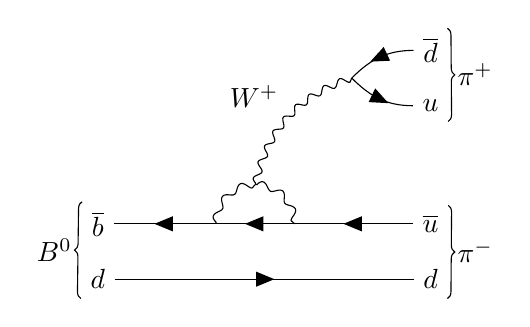
\begin{tikzpicture}\begin{feynman}
\vertex(a1){\(\overline b\)};\vertex[right=1.5cm of a1] (a2);\vertex[right=1cm of a2] (a3);\vertex[right=1.5cm of a3] (a4){\(\overline u\)};\vertex[below=2em of a1] (b1){\(d\)};\vertex[below=2em of a4] (b2){\(d\)};
%% See section 13.5 of PGF/TikZ manual
\vertex at ($(a2)!0.5!(a3)!0.5cm!90:(a3)$) (d);
%% Equivalent way to obtain (d):
%\vertex at ($(b2)!0.5!(b3) + (0, -0.5cm)$) (d);
\vertex[above=of a4] (c1){\(u\)};\vertex[above=2em of c1] (c3){\(\overline d\)};\vertex at ($(c1)!0.5!(c3)- (1cm, 0)$) (c2);\diagram* {(a4)-- [fermion] (a3)-- [fermion] (a2)-- [fermion] (a1),(b1)-- [fermion] (b2),(c3)-- [fermion,out=180,in=45] (c2)-- [fermion,out=-45,in=180] (c1),(a2)-- [boson,quarter left] (d)-- [boson,quarter left] (a3),(d) -- [boson, bend left,edge label=\(W^{+}\)] (c2),};\draw[decoration={brace}, decorate] (b1.south west)-- (a1.north west)node[pos=0.5, left] {  \(B^{0}\)};\draw[decoration={brace}, decorate] (c3.north east)-- (c1.south east)node[pos=0.5, right] {  \(\pi^{+}\)};\draw[decoration={brace}, decorate] (a4.north east)-- (b2.south east)node[pos=0.5, right] {  \(\pi^{-}\)};
\end{feynman}
\end{tikzpicture}

\def \thelable {A}
\begin{tikzpicture}
\begin{feynman}
\vertex(field);
\vertex[right=1.0cm of field](wilsoncoupling);
\vertex[right=2.0cm of wilsoncoupling](infinity);
\vertex[below=1cm of field](3gluon);
\vertex[below=1cm of 3gluon](outgoingfield);
\diagram* {(field) -- [scalar] (wilsoncoupling) -- [scalar] (infinity)};
\diagram* {(field) -- [boson] (3gluon) -- [boson] (wilsoncoupling)};
\diagram* {(3gluon) -- [boson] (outgoingfield)};
\vertex[right=2.0cm of field](auxpoint);
\vertex[below=1.5cm of auxpoint](label){\(\thelable\)};
\end{feynman}
\end{tikzpicture}
\def \thelable {B}
\begin{tikzpicture}
\begin{feynman}
\vertex(field);
\vertex[right=1.0cm of field](wilsoncoupling);
\vertex[right=2.0cm of wilsoncoupling](infinity);
\vertex[below=1cm of field](3gluon);
\vertex[below=1cm of 3gluon](outgoingfield);
\diagram* {(field) -- [scalar] (wilsoncoupling) -- [scalar] (infinity)};
\diagram* {(field) -- [boson,half left] (3gluon) -- [boson,half left] (field)};
\diagram* {(3gluon) -- [boson] (outgoingfield)};
\vertex[right=2.0cm of field](auxpoint);
\vertex[below=1.5cm of auxpoint](label){\(\thelable\)};
\end{feynman}
\end{tikzpicture}

\def \thelable {C}
\begin{tikzpicture}
\begin{feynman}
\vertex(field);
\vertex[right=1.0cm of field](wilsoncoupling);
\vertex[right=2.0cm of wilsoncoupling](infinity);
\vertex[below=1cm of field](3gluon);
\vertex[below=1cm of 3gluon](outgoingfield);
\diagram* {(field) -- [scalar] (wilsoncoupling) -- [scalar] (infinity)};
\diagram* {(field) -- [boson,half left] (wilsoncoupling)};
\diagram* {(field) -- [boson] (outgoingfield)};
\vertex[right=2.0cm of field](auxpoint);
\vertex[below=1.5cm of auxpoint](label){\(\thelable\)};
\end{feynman}
\end{tikzpicture}




\ifdefined\mainprogram{}
\else
\end{document}

\fi
\end{document}
